%% 
%% Copyright 2007, 2008, 2009 Elsevier Ltd
%% 
%% This file is part of the 'Elsarticle Bundle'.
%% ---------------------------------------------
%% 
%% It may be distributed under the conditions of the LaTeX Project Public
%% License, either version 1.2 of this license or (at your option) any
%% later version.  The latest version of this license is in
%%    http://www.latex-project.org/lppl.txt
%% and version 1.2 or later is part of all distributions of LaTeX
%% version 1999/12/01 or later.
%% 
%% The list of all files belonging to the 'Elsarticle Bundle' is
%% given in the file `manifest.txt'.
%% 

%% Template article for Elsevier's document class `elsarticle'
%% with numbered style bibliographic references
%% SP 2008/03/01

\documentclass[preprint,12pt]{elsarticle}
%\makeatletter
%\def\@author#1{\g@addto@macro\elsauthors{\normalsize%
%    \def\baselinestretch{1}%
%    \upshape\authorsep#1\unskip\textsuperscript{%
%      \ifx\@fnmark\@empty\else\unskip\sep\@fnmark\let\sep=,\fi
%      \ifx\@corref\@empty\else\unskip\sep\@corref\let\sep=,\fi
%      }%
%    \def\authorsep{\unskip,\space}%
%    \global\let\@fnmark\@empty
%    \global\let\@corref\@empty  %% Added
%    \global\let\sep\@empty}%
%    \@eadauthor={#1}
%}
%\makeatother
%% Use the option review to obtain double line spacing
%% \documentclass[authoryear,preprint,review,12pt]{elsarticle}

%% Use the options 1p,twocolumn; 3p; 3p,twocolumn; 5p; or 5p,twocolumn
%% for a journal layout:
%% \documentclass[final,1p,times]{elsarticle}
%% \documentclass[final,1p,times,twocolumn]{elsarticle}
%% \documentclass[final,3p,times]{elsarticle}
%% \documentclass[final,3p,times,twocolumn]{elsarticle}
%% \documentclass[final,5p,times]{elsarticle}
%% \documentclass[final,5p,times,twocolumn]{elsarticle}

%% For including figures, graphicx.sty has been loaded in
%% elsarticle.cls. If you prefer to use the old commands
%% please give \usepackage{epsfig}

%% The amssymb package provides various useful mathematical symbols
\usepackage{amssymb}
\usepackage{amsthm}
%\usepackage[pdftex]{graphicx}
\usepackage{color}
\usepackage{listings}
\usepackage{subfig}
\usepackage{float}
\usepackage{longtable}
\usepackage{supertabular}
\usepackage{pbox}
\usepackage{amsmath}
\newcommand{\verbatimfont}[1]{\def\verbatim@font{#1}}%

%\renewcommand{\baselinestretch}{.97}

%\usepackage{tablefootnote}
%
%
%\usepackage{booktabs}
%\captionsetup[table]{position=top,labelfont={sc},textfont={sl}}
%\renewcommand{\thetable}{\Roman {table}}

% correct bad hyphenation here
%\definecolor{gray}{rgb}{255,255,255}

\lstloadlanguages{HTML,XML}
\lstset{%
language=XML,
frame=tb,
framerule=1pt,
rulesep=0pt,
basicstyle=\scriptsize,
showstringspaces=false,
numbers=left,
numberstyle=\scriptsize,
stepnumber=1,
numbersep=2pt,
%backgroundcolor=\color{gray},
showspaces=false,
showtabs=false,
escapeinside={\%*}{*)}
}

\mathchardef\mhyphen="2D


\hyphenation{a-no-ny-mi-ty VA-NET}
\newtheorem{definition}{Definition}
\newcommand{\protocolname}{$ASAP$-V} 
%% The amsthm package provides extended theorem environments
%% \usepackage{amsthm}

%% The lineno packages adds line numbers. Start line numbering with
%% \begin{linenumbers}, end it with \end{linenumbers}. Or switch it on
%% for the whole article with \linenumbers.
%% \usepackage{lineno}

\journal{Information Sciences}

\begin{document}

\begin{frontmatter}

%% Title, authors and addresses

%% use the tnoteref command within \title for footnotes;
%% use the tnotetext command for theassociated footnote;
%% use the fnref command within \author or \address for footnotes;
%% use the fntext command for theassociated footnote;
%% use the corref command within \author for corresponding author footnotes;
%% use the cortext command for theassociated footnote;
%% use the ead command for the email address,
%% and the form \ead[url] for the home page:
%% \title{Title\tnoteref{label1}}
%% \tnotetext[label1]{}
%% \author{Name\corref{cor1}\fnref{label2}}
%% \ead{email address}
%% \ead[url]{home page}
%% \fntext[label2]{}
%% \cortext[cor1]{}
%% \address{Address\fnref{label3}}
%% \fntext[label3]{}

\title{$ASAP$-V: A Privacy-preserving Authentication and Sybil detection Protocol for VANETs}


%\author[label1]{Thiago de Sales\corref{cor1}} 
%\ead{thiago.sales@ee.ufcg.edu.br} 
%\address[label1]{% 
%Aprigio Veloso Street, n� 882\\ 
%Electrical Engineering and Informatics Center (CEEI)\\ 
%Federal University of Campina Grande (UFCG)\\ 
%58429 900 Campina Grande, PB, Brazil\\ 
%Tel: +55-82-3091-5397\\ 
%} 
%\cortext[cor1]{Corresponding Author} 
% 
%\author[label2]{Angelo Perkusich} 
%\ead{hani@cefala.org} 
%\address[label2]{CEFALA--CPDE--UFMG} 
% 
%\author[label1]{Anna Helena Reali Costa\fnref{money}} 
%\ead{anna.reali@poli.usp.br} 


%
% \author{Thiago M. de Sales\corref{cor1}\fnref{label2}, Angelo Perkusich\fnref{label2}}
% \ead{thiagobruno@embedded.ufcg.edu.br}
% \ead[url]{home page}
% \fntext[label2]{Electrical Engineering and Informatics Center, Federal University of Campina Grande, UFCG, Brazil.}
% \cortext[cor1]{thiago.sales@ee.ufcg.edu.br}
% \address{Addressss\fnref{label3}}
% \fntext[label3]{Intuit, Inc. USA.}



\author[label1]{Thiago Bruno M. de Sales\corref{cor1}}
\ead{thiago.sales@ee.ufcg.edu.br}
\author[label1]{Angelo Perkusich}
\ead{perkusich@dee.ufcg.edu.br}
\author[label1]{Leandro Melo de Sales}
\ead{leandro@embedded.ufcg.edu.br}
\author[label1]{Hyggo Oliveira de  Almeida}
\ead{hyggo@dsc.ufcg.edu.br}
\author[label1]{Gustavo Soares}
\ead{gsoares@computacao.ufcg.edu.br}
\address[label1]{Embedded Systems and Pervasive Computing Laboratory, Federal University of Campina Grande, Campina Grande, PB, Brazil}

\author[label2]{Marcello de Sales}
\ead{Marcello\_deSales@intuit.com}
\address[label2]{Intuit, Inc. San Diego, C.A, USA}
\cortext[cor1]{Corresponding author}


%% use optional labels to link authors explicitly to addresses:
% \author[label1,label2]{Thiago de Sales\corref{cor1}}
% \author[label1]{Angelo Perkusich}
% \author[label1]{Hyggo Almeida}
% \author[label1, label2]{Leandro de Sales}
% \author[label1]{Gustavo Soares}
% \author[label3]{Marcello de Sales}
%\address[label1]{Electrical Engineering and Informatics Center, Federal University of Campina Grande, UFCG, Brazil.}
%\address[label2]{Computer Science Department, Federal University of Alagoas, UFAL, Brazil.}
%\address[label3]{Intuit, Inc. USA.}
%\cortext[cor1]{thiago.sales@ee.ufcg.edu.br}

%\author{Thiago de Sales, Angelo Perkusich}
%
%\address{label1}{Federal University of Campina Grande, Brazil}
%\address{label2}{Federal University of Alagoas, Brazil}

%Therefore, it may decrease service reliability and impact network performance. 
%The anonymity set concept is suggested to detect \textit{sybil} attacks without compromising users' privacy. What is more, \protocolname~does not require a fixed infrastructure during \textit{sybil} attack detection time. 
%In addition, we measured our anonymous communication model, which shows its efficiency to balance between privacy and vehicle's information disclosure
\begin{abstract}
Node authentication, non-repudiation and anonymous communication are key roles to provide security in Vehicular Ad Hoc Networks (VANETs). On the other hand, the trade-off between authentication/non-repudiation and anonymous communication may lead to a harmful type of network attack called \textit{sybil} attack. In such an attack, a malicious node behaves as if it is a large number of nodes. In this paper, we propose an anonymous authentication and \textit{sybil} attack detection protocol for VANETs called \protocolname. Experimental results suggest that \protocolname~is more robust against \textit{sybil} attacks, with lower average detection time than the state-of-art works, also without false-positive and false-negative detections.
\end{abstract}

\begin{keyword}

VANET \sep Security \sep Authentication \sep Privacy \sep Sybil Attack
%% keywords here, in the form: keyword \sep keyword
% - provide a maximum of 6 keywords, using American spelling and avoiding general and plural terms and multiple concepts (avoid, for example, 'and', 'of'). Be sparing with abbreviations: only abbreviations firmly established in the field may be eligible. These keywords will be used for indexing purposes.

%- Table footnotes
%- Indicate each footnote in a table with a superscript lowercase letter

%- TIFF (or JPEG): Color or grayscale photographs (halftones), keep to a minimum of 300 dpi.
%TIFF (or JPEG): Bitmapped (pure black & white pixels) line drawings, keep to a minimum of 1000 dpi.
%TIFF (or JPEG): Combinations bitmapped line/half-tone (color or grayscale), keep to a minimum of
%500 dpi.

%- Please make sure that artwork files are in an acceptable format (TIFF (or JPEG), EPS (or PDF), or
%MS Office files) and with the correct resolution. If, together with your accepted article, you submit
%usable color figures then Elsevier will ensure, at no additional charge, that these figures will appear in
%color on the Web (e.g., ScienceDirect and other sites) regardless of whether or not these illustrations
%are reproduced in color in the printed version. For color reproduction in print, you will receive
%information regarding the costs from Elsevier after receipt of your accepted article. Please
%indicate your preference for color: in print or on the Web only. For further information on the
%preparation of electronic artwork, please see http://www.elsevier.com/artworkinstructions.

%- Tables
%Number tables consecutively in accordance with their appearance in the text. Place footnotes to tables
%below the table body and indicate them with superscript lowercase letters. Avoid vertical rules. Be
%sparing in the use of tables and ensure that the data presented in tables do not duplicate results
%described elsewhere in the article.

%- Reference linking: Use of the DOI is encouraged.

%- REVER O Reference Style

%- REVER O Submission checklist quando for submeter

%% PACS codes here, in the form: \PACS code \sep code

%% MSC codes here, in the form: \MSC code \sep code
%% or \MSC[2008] code \sep code (2000 is the default)

%- Present simple formulae in the line of normal text where possible and use the solidus (/) instead of a horizontal line for small fractional terms, e.g., X/Y. In principle, variables are to be presented in italics.


\end{keyword}

\end{frontmatter}

\section{Introduction}

The Vehicular Ad Hoc Network (henceforth VANET) is an emerging type of Mobile Ad Hoc Network (MANET) that aims at providing vehicular safety applications, optimized vehicular traffic routing, and real-time applications for drivers and passengers, such as mobile infotainment~\cite{al2013comprehensive}. Vehicles act as mobile nodes\footnote{We use the terms vehicles, nodes and cars interchangeably.} that can send message to other vehicles and to road side units (RSUs), which are fixed infrastructures along the roads that may provide vehicle connectivity in sparse or low density areas. The communication between vehicles is called V2V (Vehicle-to-Vehicle), while the communication between vehicle and RSU is called V2I (Vehicle-to-Infrastructure). The IEEE 802.11p~\cite{ieee11802} standard is used for wireless communication.

%In VANET, vehicles communicate by means of the North American Dedicated Short-Range Communication (DSRC) standard, that employs the IEEE 802.11p~\cite{ieee11802} for wireless communication. Vehicles may send two types of messages: periodic (or beacon), and event-driven messages. The former allows a vehicle to announce its current position, speed, and direction to neighbors, allowing other vehicles to perceive and predict the kinematics of the vehicle. The latter may inform sporadic events, such as road hazardous warnings (on-road obstacles, icy surfaces, weather conditions, to name a few).	

The concepts behind VANET are bringing new challenges to a diverse of network research areas, including security~\cite{gillani2013survey}. Security has been considered a critical concern due to VANET's open wireless nature, since no authentication and association procedures are in 802.11p. Thus, VANET requires fundamental security aspects in the application layer such as the vehicles' message authentication and non-repudiation. 

%In this context, there have been a lot of new authentication approaches~\cite{riley2011survey} for VANET, which basically may include the two common cryptography key models, such as symmetric and/or asymmetric keys though Public Key Infrastructure (PKI)~\cite{keys-distro1}, \cite{keys-distro2-thesis}, \cite{MolinaGil2014172}, and \cite{keys-distro8}, as well as the group~\cite{lin2007gsis} and identity-based signature schemes \cite{authentication-id-based1}.

However, authentication and non-repudiation require a one-to-one correspondence between vehicle and identity, which may allow a malicious entity to build a vehicle's route profile. This may  compromise users' privacy and lead to several user safety problems such as kidnapping, and undesirable tracking for mobile advertisement~\cite{mix-zone-vanets}. However, through a simple and secure, yet powerful mathematical and logical analysis, researchers \cite{haas2010impact} identified that the more suitable identity assignment to vehicles is to each one to store multiple identities (also called multiple \textit{pseudonyms}), without sharing any identity with others, each identity unique to each vehicle. 

%In order to secure users' location privacy, there are essentially three types of identity distribution: \textit{i)} all vehicles share the same identity (same key); \textit{ii)} each vehicle keeps multiple identities and certain groups of vehicles share a set of identities; and \textit{iii)} each vehicle stores multiple identities (also called multiple \textit{pseudonyms}), without sharing any identity, which are unique to each vehicle. Through a simple and secure, yet powerful mathematical and logical analysis, researchers identified that the more suitable identity assignment was the last one~\cite{haas2010impact}, which leads to a reasonable users' privacy and fast, yet secure revocation of cryptography keys.

%In order to secure users' location privacy, there are essentially three types of identity distribution: \textit{i)} all vehicles share the same identity (same key); \textit{ii)} each vehicle keeps multiple identities and certain groups of vehicles share a set of identities; and \textit{iii)} each vehicle stores multiple identities (also called multiple \textit{pseudonyms}), without sharing any identity, which are unique to each vehicle. Through a simple and secure, yet powerful mathematical and logical analysis, researchers identified that the more suitable identity assignment was the last one~\cite{haas2010impact}, which leads to a reasonable users' privacy and fast, yet secure revocation of cryptography keys.

Initially proposed by Raya et. al.\cite{keys-distro1}, there have been many other multiple-pseudonym-based approaches for securing location privacy in VANET~\cite{keys-distro2-thesis}, \cite{keys-distro8}, \cite{calandriello2007efficient} and  \cite{sun2010efficient}. Many researchers adopt the concept of Mix Zones~\cite{mix-zone} to prevent malicious entities from linking different vehicle's pseudonyms~\cite{lu2012pseudonym}, \cite{mix-zone-vanets}, \cite{buttyan2007effectiveness}, \cite{caravan}, \cite{buttyan2009slow} and \cite{mix-zone-motion}. In this case, the main goal is to spatially and temporally build groups of vehicles in order to allow them to change their pseudonyms without compromising users' privacy.

Even so, the multiple-pseudonym approach leads to a simple, but harmful type of network attack called a \textit{sybil} attack~\cite{sybil}. In \textit{sybil} attacks, a malicious node behaves as if it is a large number of nodes. Since a vehicle may have multiple valid identities to control its privacy, a malicious vehicle can send multiple messages with different identities to inform false events in VANETs. 

Some examples include false on-road obstacles and false emergency braking warning along a road, or creating an illusion of traffic congestion through beacon messages by claiming to be at different locations. The presence of a \textit{sybil} node increases packet loss, and decrease the packet delivery ratio and the aggregated throughput due to incorrect routing paths~\cite{sybil-impact3}, \cite{sybil-impact2} and \cite{sybil-attack-impact-routing1}. When a vehicle is not a \textit{sybil} node, it is called \textit{legitimate vehicle}.

%Figure~\ref{fig:sybilscenario1} illustrates a \textit{sybil} attack scenario that may defeat routing 	algorithms. Suppose that vehicles A and D need to send messages to each other, but their wireless signal strength are not enough to reach each other. Therefore, they need to send each message to nearby vehicles through geographical-based routing algorithms, such as GPSR (\textit{Greedy Perimeter Stateless Routing})~\cite{greedy-routing, routing6} and MDDV (\textit{Mobility-centric Data Dissemination Algorithm for Vehicular Networks})~\cite{routing8}. Also suppose that vehicle \textit{e'} is a \textit{sybil} node that also sends beacon messages with two other different locations with identities $e''$ and $e'''$. Thus, vehicles \textit{a} and \textit{d} will send messages to $e''$  ($a \rightarrow e'' \rightarrow d$) and $e'''$ ($d \rightarrow e''' \rightarrow a$), respectively. Therefore, vehicle \textit{e'} will receive the messages and may change their contents, or simply drop them. 
%
%\begin{figure}[ht]
%\centering
%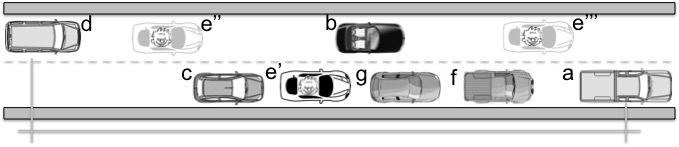
\includegraphics[width=3.5in, height=0.8in]{figures/cenario-sybil-5-en.jpg}
%\caption{Sybil vehicle \textit{e'} sends three different beacon messages with three identities.}
%\label{fig:sybil2}
%\end{figure}


%\begin{figure}[ht]
%\centering
%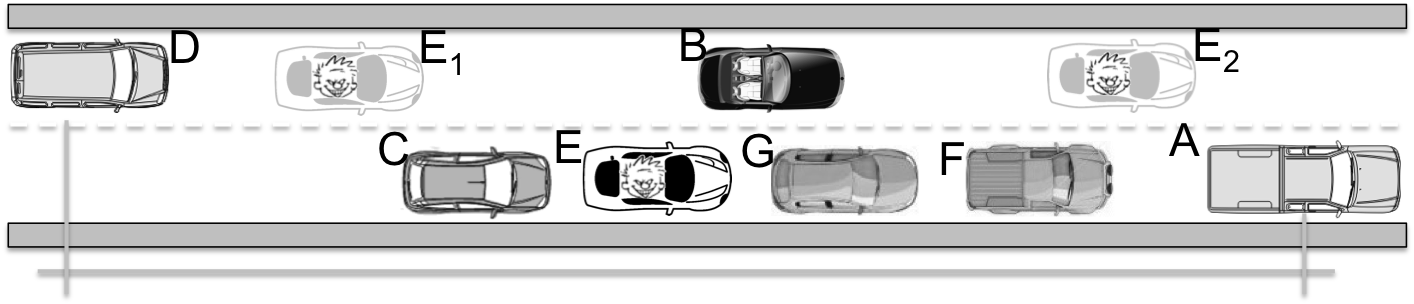
\includegraphics[width=5.5in]{figures/cenario-sybil-5-en.png}
%\caption{Scenario 1: \textit{sybil} attacks through beacon messages. Sybil vehicle E may drop all messages from vehicles A and D.}
%\label{fig:sybilscenario1}
%\end{figure}


To avoid a vehicle from keeping, at the same time, multiple identities in multiple-pseudonym-based approaches, other works propose a single vehicle to store only one identity at a time~\cite{keys-distro4}, \cite{keys-distro7} and \cite{profile-generation1}. To change its identity, each vehicle requests from the RSUs along the road, one new identity that is valid only in the region where the RSU is responsible for. These approaches lack flexibility and they are highly dependable on the RSUs deployment methods~\cite{rsu-placement1}. 

%Other approaches explore the RSU and Certificate Authority (CA) to detect \textit{sybil} attacks~\cite{p2dap2} and \cite{p2dap}, as well as the relationship between time and space~\cite{sybil-time-space1} and \cite{sybil-time-stamp1} and the use of neighboring vehicles to filter malicious vehicles~\cite{sybil-neighborhood1} and \cite{sybil-neighborhood3}. Nonetheless, due to the tradeoff between \textit{sybil} detection attacks and privacy-preserving authentication, these approaches suffer from \textit{false-negative} \textit{sybil} attack detections, when a malicious vehicle is not detected as one. 

Based on a deep investigation of the state of the art approach, this paper proposes a decentralized privacy-preserving authentication and \textit{sybil} attack detection protocol for VANETs called~\protocolname~(\textit{Authentication and Sybil Attack detection Protocol for VANETs}). The authentication process is based on the multiple-pseudonym approach to provide location privacy for the users. Non-repudiation is also achieved through the Group Signature Scheme~\cite{group-sign}. Our approach uses the anonymity set theory~\cite{k-anonymity} in a multilevel fashion to detect and avoid \textit{sybil} attacks, while still providing users' privacy control. 

%The proposed solution does not require a fixed infrastructure during the \textit{sybil} attack detection time, nor does it require third-party services such as trust and reputation systems~\cite{trust}. Instead, the \textit{sybil} detection is coordinated through the vehicles in the vicinity. We evaluated our approach using an extension of the CSP (Communication Sequencial Process) algebra called Rank Function Theorem~\cite{schneider1996security},\cite{schneider1998verifying}, which proves that our multiple-pseudonym authentication approach is secure, and the \textit{sybil} detection protocol through simulated experiments. Finally, we measured our anonymous communication model, which shows its efficiency to balance between privacy and vehicle's information disclosure.

The contributions of this paper are summarized as follows:

\begin{itemize}
	\item a new privacy-preserving authentication and \textit{sybil} detection protocol;
	\item decentralization of the \textit{sybil} detection approach, which does not require a fixed infrastructure during detection time;
	\item an approach without false-negative and false-positive \textit{sybil} detections, even without the support of an infrastructure;
	\item it is able to detect \textit{sybil} attacks from both beacon and event-driven messages;
	\item our results suggest that the detection protocol provides lower average \textit{sybil} attack detection time than the state-of-the-art approaches. 
\end{itemize}

The remainder of the paper is organized as follows: Section~\ref{sec:solution} details the proposed privacy-preserving authentication and \textit{sybil} detection approach. Section~\ref{sec:results} discusses the experiments and results of the approach, while Section~\ref{sec:related} discusses the related works about privacy-preserving \textit{sybil} detection attacks. Finally, Section~\ref{sec:conclusion} presents the conclusions and future work.

\section{A Privacy-preserving Authentication and Sybil Attack Detection Protocol for VANET}
\label{sec:solution}

This section details the \protocolname~architecture. The goal is to provide strong privacy-preserving authentication and non-repudiation while detecting \textit{sybil} attacks. 

%\subsection{The Threat Model}
%
%The two main threats that we need to cope with are the \textit{sybil} attack, and the potential violation of the driver's privacy. According to the Raya taxonomy~\cite{keys-distro1}, the former threat may be launched from malicious users classified as \textit{insider} (users with authenticated vehicle), \textit{malicious} or \textit{rational} (users that aim to harm or just to seek personal profit, respectively), \textit{active} (users that can generate authenticated messages), and \textit{local} (users that are limited in scope). On the other hand, the latter threat may be launched from a malicious entity classified as an \textit{insider} or \textit{outsider} (an intruder), \textit{rational}, \textit{passive} (users that only eavesdrop on the wireless channel), and \textit{extended} (users that control several sensors that are scattered across the network).

\subsection{The \protocolname~protocol description}

%The \protocolname~uses the concepts of pseudonyms and the anonymity set theory for protecting users' privacy, as well as the group signature scheme for providing non-repudiation. To detect \textit{sybil} attacks while preserving users' privacy, the \protocolname~organizes the vehicles into multiple anonymity sets organized in a multilevel architecture. This way, each vehicle shares a set of attributes with other vehicles, but it must have at least one attribute that differs from other vehicles in a given period of time.

The \protocolname~protocol is divided into four phases: the registration phase (Phase 1); the temporary identity (pseudonym) assignment phase (Phase 2); the \textit{sybil} detection phase (Phase 3); and the prosecution phase (Phase 4). For the next sections, Table~\ref{tab:nomenclature} summarizes the notations for the protocol description.

\begin{longtable}{ p{.15\textwidth} p{.70\textwidth} } 
\caption{Notations.} % needs to go inside longtable environment
\label{tab:nomenclature} \\ \hline
Symbol & Description  \\
\hline
\endfirsthead
\multicolumn{2}{c}%
{\tablename\ \thetable\ -- \textit{continued from previous page}} \\
\hline
Symbol & Description  \\
\hline
\endhead
\hline \multicolumn{2}{r}{\textit{continued on next page}} \\
\endfoot
\hline
\endlastfoot
$v_{c}$ & A Vehicle \textit{c}. \\
$RSU_{n}$ & The $n^{th}$ RSU along the road. \\ 
$cert_{a}$ & Digital certificate of an entity \textit{a}. \\ 
$k^{+}_{a, n}$ & The \textit{a}'s $n^{th}$ public key. \\ 
$k^{-}_{a, n}$ & The \textit{a}'s $n^{th}$ private key. \\ 
$cert_{a, n}$ & The \textit{a}'s $n^{th}$ public key digital certificate.\\  
$TK_{a}$ & \textit{a}'s set of temporary public/private key pairs (pseudonyms).\\  
$gsk_{c}$ & Group signing key of vehicle \textit{c}.\\ 
$gpk$ & A group public key.\\ 
$grt_{a}$ & Group revocation token of vehicle \textit{a}.\\ 
$RL$ & List of revoked \textit{group revocation tokens}.\\ 
$tmp$ & Current timestamp. \\ 
$tmp_{ctn}$ & The timestamp that the content \textit{ctn} was digitally signed. \\ 
$threshold_{X}$ & \pbox{20cm}{Denotes the maximum (X = \textit{max}) or minimum \\ (X = \textit{min}) timestamp value to define time intervals.} \\ 
$Signed^{ctn}_{a}$ & Entity \textit{a} signed content \textit{cnt}. \\ 
$Sign(\bullet)$ & A digital signature function. \\
$a \Rightarrow b: ctn$ & Entity \textit{a} sends content \textit{ctn} to entity \textit{b}.\\ 
$Verify(\bullet)$ & Cryptography verification function. \\ 
$E(\bullet)$ & An encryption function. \\ 
$D(\bullet)$ & A decryption function. \\ 
$sybil_{v_{c}}$ & Vehicle $v_{c}$ is a \textit{sybil} node. \\ 
\end{longtable}


The \protocolname~protocol runs in a system SV, defined as:

\begin{center}
$SV = \langle V, RSU, ca \rangle$,
\end{center}

\noindent
such that,

\begin{itemize}
	\item  $V = \{v_{0}, v_{1}, ..., v_{p}\}$ is the set of all registered vehicles ($p \in \mathbb{N})$;
	
	\item $RSU = \{RSU_{0}, RSU_{1}, RSU_{2}, ..., RSU_{r}\}$ is the set of Road Side Units (RSUs) registered in SV. The RSUs share a unique public/private key pair $(k^{+}_{RSU}, k^{-}_{RSU}) \in K_{RSU}$, and $cert_{RSU}$ denotes the RSUs' public key digital certificate;
	
	\item \textit{ca} denotes a Certificate Authority (CA), which is responsible for managing key materials and for storing vehicles' and RSUs' data in SV. The tuple $\langle (k^{-}_{CA}, k^{+}_{CA}, cert_{CA}),$ \textit{gmsk}, K-AS $\rangle$ represents a CA such that $k^{+}_{CA}$ and $k^{-}_{CA}$ denote its public and private key pair, and $cert_{CA}$ the public key's digital certificate. A CA belongs to the government and is the only entity that can trace vehicles' owners identities from vehicles' messages. This procedure is only possible through CA's group management signing key \textit{gmsk}. Finally, K-AS denotes the set of Anonymity Sets~\cite{privacytecterminology1}, discussed in Section~\ref{sec:phase1}.
\end{itemize}

\subsection{Vehicle Registration and Authentication (Phase 1)}
\label{sec:phase1}
Figure~\ref{fig:vehicle-registration} depicts the registration phase. A CA is responsible for managing the unique vehicles' identities by using the Group Signature Scheme~\cite{group-sign}. A vehicle $v_{c}$  has its own group signing key ($gsk_{c}$) and also shares the group public key (\textit{gpk}) with others. Vehicles also store the digital certificate of the CA ($cert_{CA}$) and the digital certificate of the road side units ($cert_{RSU}$). Moreover, each vehicle receives a set $TK_{c}$ of \textit{w} temporary (identities, or pseudonyms) asymmetric key pairs and their digital certificates ($k^{+}_{c,i}$, $k^{-}_{c,i}$, $cert_{c,i}$, $1 \le i \le w$). In case of judicial disputes, the CA is the only entity that can trace the original vehicle identity from a given message $m_{c}$ using its group manager secret key (\textit{gmsk}). 


%Figure~\ref{fig:vehicle-registration} summarizes the process of vehicle registration and authentication as the first step of the execution of the \protocolname~protocol. A CA is responsible for managing the unique identities of the vehicles by using the group signature scheme. Each vehicle has its own group sign key ($gsk_{c}$) and also shares the group public key (\textit{gpk}) with others. Vehicles also store the digital certificate of the CA ($cert_{CA}$) and the digital certificate of the roadside units ($cert_{RSU}$). Moreover, each vehicle receives one temporary (pseudonym) asymmetric key pair and its certificate ($k^{+}_{c,1}$, $k^{-}_{c,1}$, $cert_{c,1}$). In case of judicial disputes, the CA is the only entity that can trace the original vehicle identity from a given message using its group manager secret key (\textit{gmsk}).

\begin{figure}[ht]
\centering
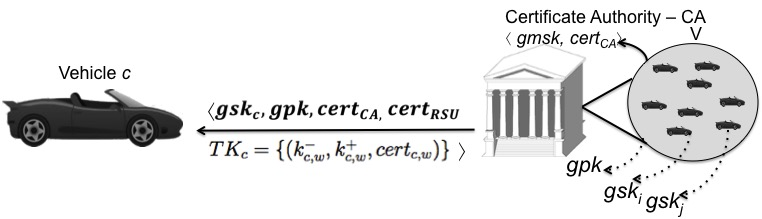
\includegraphics[width=4in, height=1.1in]{figures/registro-veiculo-en.jpg}
\caption{Vehicle registration and authentication.}
\label{fig:vehicle-registration}
\end{figure}

The second step of the registration phase aims to cluster each vehicle into multiple sets of vehicles $AS_{i,j}$ ($i, j \in \mathbb{N}^{*}; 1 \le i \le m, 1 \le j \le n$). Each set $AS_{i,j}$  has all of the properties of the anonymity set theory. According to Figure~\ref{fig:multilevel-arch}, the anonymity sets $AS_{m,n}$ are organized in \textit{m} levels, where each level has \textit{n} anonymity sets. The proposed multilevel anonymity set architecture has the following properties, which from 1 to 3 aim at protecting users privacy, while property 4 aims at detecting \textit{sybil} attacks:

\begin{enumerate}
	\item Let K-AS = \{$AS_{1,1}$, $AS_{1,2}$, ..., $AS_{1,n}$, ...,  $AS_{2,1}$, $AS_{2,2}$, ..., $AS_{2,n}$, ..., $AS_{m,n}$\} be the set of all anonymity sets;
	
	\item Each vehicle must belong to at least \textit{k} sets ($1 \textless k \textless n$) in each level. $AS_{c}$ denotes the set of all anonymity sets that vehicle $v_{c}$ belongs to ($AS_{c} \subseteq K \mhyphen AS$). 
	
	%For instance, $AS_{c} = \{AS_{1,1}, AS_{1,3}, AS_{1,12}, AS_{1,22}, AS_{1,35}, AS_{2,5},$ $AS_{2,9}, ..., AS_{m,n}\}$ if it belongs to anonymity sets $AS_{1,1}, AS_{1,3}$, and thus, $v_{c} \in AS_{1, 1} \wedge v_{c} \in AS_{1, 3} \wedge ... \wedge v_{c} \in AS_{m,n}$;
	
\item Each anonymity set $AS_{i,j}$ has a digital certificate $cert_{AS_{i,j}}$ signed by CA, that is, $Signed^{cert_{AS_{i,j}}}_{CA}$. Thus, if vehicle $v_{c}$ belongs to $AS_{i,j}$, then $v_{c}$ must store $cert_{AS_{i,j}}$. Formally, $v_{c} \in AS_{i,j} \rightarrow cert_{AS_{i,j}} \in$ $CERT_{AS_{c}}$ \{$i, j \in \mathbb{N}$, $1 \le i \le m$ e $1 \le j \le n$\}, such that:
	
	\begin{enumerate}
		\item $CERT_{AS_{c}}$ is the set of all anonymity sets' digital certificates in which the vehicle $v_{c}$ belongs to; and,
	
		\item for a given time interval \textit{t}, a vehicle $v_{c}$ must choose a subset $CERT^{t}_{AS_{c}}$ of anonymity set digital certificates ($CERT^{t}_{AS_{c}} \subseteq CERT_{AS_{c}}$) that comprises only one digital certificate per level.
	\end{enumerate}
	
	\item Any two vehicles $v_{c}$ and $v_{c'}$ in $AS_{1,j}$ must not belong to the same anonymity set of some lower level. Formally\footnote{The symbol $\oplus$ represents an exclusive-or operator.}, $\forall v_{c}, v_{c'} \in AS_{1, j},$  $\exists$ $i$ $(\forall$ $r$ $(v_{c} \in AS_{i,r} \oplus v_{c'} \in AS_{i,r} )) $ $ \{i, j, r \in \mathbb{N} : 1 < i \le m, 1 \le j \le n, 1 \le r \le n\}$. Therefore, $CERT^{t}_{AS_{c}} - CERT^{t}_{AS_{c'}} \neq \emptyset$. 
\end{enumerate}

\begin{figure}[ht]
\centering
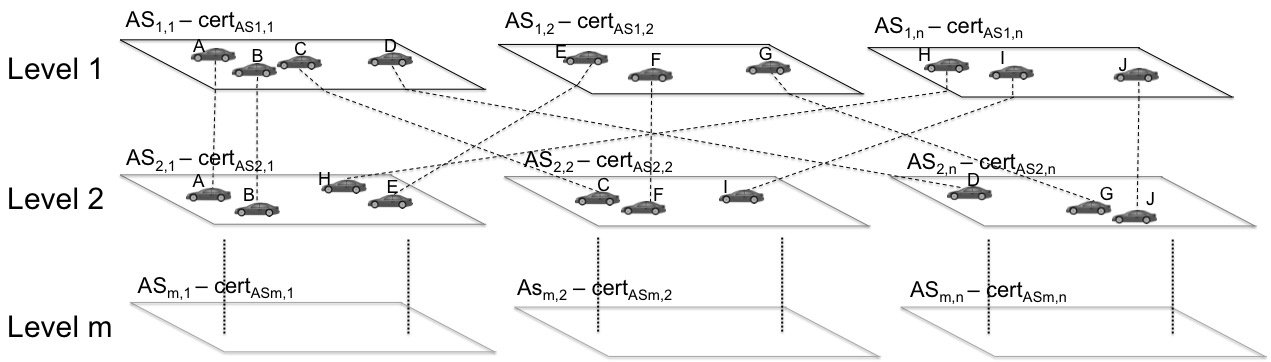
\includegraphics[width=5.5in, height=1.3in]{figures/vehicle-groups3-en.jpg}
\caption{The Multilevel \protocolname~Architecture.}
\label{fig:multilevel-arch}
\end{figure}


Finally, a vehicle $v_{c}$ is represented by the following tuple:

\begin{center}
$v_{c} = \langle (gsk_{c}, gpk), TK_{c}, AS_{c}, CERT_{AS_{c}}  \rangle$.
\end{center}


\subsection{Temporary Key Assignment (Phase 2)}
\label{sec:phase2}

In order to protect users' privacy, the multiple-pseudonym approach is used, and the second phase is responsible for managing pseudonym assignments to vehicles. In the \protocolname~protocol, cryptography asymmetric key pairs represent vehicle pseudonyms. For instance, the key pair $k^{+}_{c, i}/k^{-}_{c, i}$ and its digital certificate $cert_{c,i}$ is the $i^{th}$ pseudonym of the vehicle $v_{c}$. Vehicles obtain temporary keys from authenticated RSUs available along the roads. 

We modeled the proposed pseudonym renewal protocol using the CSP (Communication Sequencial Process) notation. However, before diving into the details of the protocol's authentication properties in CSP notation, we first give an overview of such protocol, as illustrated in Figure~\ref{fig:renewalprotocol}:

\begin{figure}[ht]
\centering
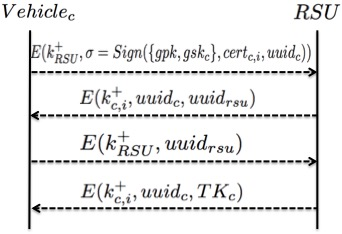
\includegraphics[scale=.45]{figures/asapvrenewalprotocol.jpg}
\caption{Pseudonym renewal protocol.}
\label{fig:renewalprotocol}
\end{figure}

\begin{itemize}
	\item In Step 1, a vehicle $v_{c}$ requests the set of temporary keys from a given $RSU$. The vehicle $v_{c}$, through the group signature schema, signs its $i^{th}$ temporary digital certificate ($cert_{c,i}$) and a random UUID (\textit{Universely Unique IDentifier}) value, which generates the group signature $\sigma$. The \textit{UUID} is a 128-bit identifier value and, within the context of ASAP-V protocol, it is used as a nonce value. Moreover, the vehicle $v_{c}$ encrypts the signature $\sigma$ using $RSU$'s public key, which generates the authentication request message;
		
	\item  In Step 2, the $RSU$ checks two parameters: first, it decrypts the received message by using its private key $k^{-}_{RSU}$. Then, it verifies if the group revocation token ($grt_{c}$) of vehicle $v_{c}$ is not in the Revocation List (RL) and if the message's timestamp (the time the request was  sent) is within a reasonable threshold in order to avoid replay attacks~\cite{replay-attack}. The \textit{Verify} function represents this process and is formally described in the Equation~\ref{eq:etapa21}. The CA is responsible for periodically sharing an updated version of RL, which is detailed in Section~\ref{sec:phase4}.

	\begin{equation} 
	\label{eq:etapa21}
		Verify(gpk, \sigma, payload_{c}) = valid \leftrightarrow grt_{c} \notin RL \wedge (\textit{tmp} - tmp_{\sigma} \le threshold_{max})
	\end{equation}			
	
	If valid, the RSU creates a new UUID value ($uuid_{rsu}$) and returns to the vehicle, which aims at allowing vehicle's authentication and avoiding \textit{man-in-the-middle} attacks. The RSU encrypts the received $uuid_{c}$ as well as the new UUID value with the $i^{th}$ vehicle public key $k^{+}_{c,i}$, which is available in the vehicle's $i^{th}$ digital certificate, received in the request message in Step 1. This response message is then sent back to $v_c$.
	
	\item In Step 3, the vehicle checks if the received UUID is the same as it sent previously. If so, $v_{c}$ returns the received UUID ($uuid_{rsu}$) by encrypting it with the RSU's public key.
	
	\item In Step 4, the RSU checks if the proposed UUID ($uuid_{rsu}$) is the same as it had sent in Step 2. If so,  the RSU has authenticated vehicle $v_{c}$. Hence, the $RSU$ generates the new set of keys $TK_{c} = \{ (k^{+}_{c,1}/k^{-}_{c,1}), (k^{+}_{c,2}/k^{-}_{c,2}), (k^{+}_{c,3}/k^{-}_{c,3})..., (k^{+}_{c,w}/k^{-}_{c,w})\}$ for vehicle $v_{c}$ and authenticates each key. Therefore, we have $Signed^{cert_{c,i}}_{RSU}$:
	
	\begin{equation}
\label{eq:etapa22}
	\forall k^{+}_{c,i} \in TK_{c} (1 \le i \le w), Sign(k^{-}_{RSU}, k^{+}_{c,i}) = cert_{c,i}.
\end{equation}

	Finally, the $RSU$ returns the new set of temporary keys  $TK_{c}$ to the vehicle $v_{c}$ by encrypting the message with the $i^{th}$ $v_{c}$'s temporary public key received in Step 1, and the $v_{c}$'s $UUID_c$ value. Vehicle $v_{c}$ accepts $TK_c$ if, and only if, $UUID_c$ received from RSU is the same as it sent in Step 1. Each key pair and its digital certificate represent a $v_{c}$'s temporary identity, also called pseudonym.
	
\end{itemize}

Vehicles must store all anonymity set digital certificates and temporary keys in a tamper-resistant Hardware Security Module (HSM), also known as tamper-proof device (TPD). This avoids malicious users from copying keying material that belongs to other vehicles. 

%A TPD is also responsible for signing messages on behalf of the vehicle's applications, as well as to check message authenticity received from other vehicles and to manage the change of pseudonyms. 

%It is important to point out that IEEE 1609.2, which describes all security aspects of the Wireless Access for Vehicular Environment (WAVE) architecture, also emphasizes that whenever practical, keying material must be protected from exposure in a TPD. Therefore, the availability of such device is an essential component to provide security services in VANETs.

%\begin{figure}[ht]
%\centering
%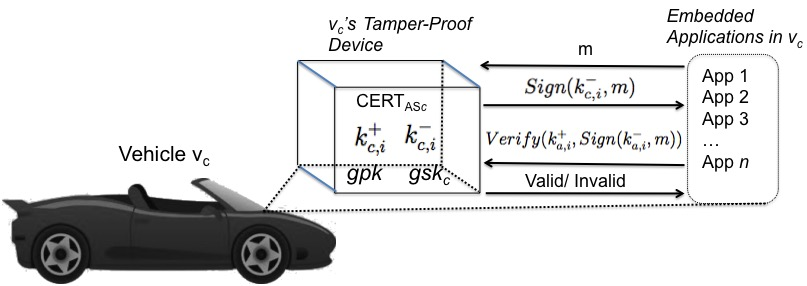
\includegraphics[scale=.35]{figures/tamper-proof-and-applications.jpg}
%\caption{A tamper-proof device (TPD), which goes inside of a vehicle, stores key materials, while applications request message digital signatures, digital signature authenticity checking and decryption, as well as pseudonym management.}
%\label{fig:tamper-proof}
%\end{figure}

We now model the pseudonym renewal protocol as a network and detail the authentication property for this network as a trace specification. Within this context, Schneider~\cite{schneider1998verifying} proposed an extension for CSP and introduced additional control events known as signals. These signal events are used in trace specifications to express the authentication goals of a protocol. Therefore, these signal events will be useful to show the correctness of the pseudonym renewal protocol, as will be discussed in Section~\ref{sec:authenticationCorrectness}. 

The following CSP specification represents a vehicle process during the pseudonym renewal protocol execution. The signal $Running\_Vehicle.v_c.rsu$ indicates that the vehicle $v_{c}$ is aware of its involvement in a run with the road side unit (rsu) and the nonce $uuid_c$ makes part of this run.
\\

\parbox[t]{1.2\textwidth}{$Vehicle_c(v_c, uuid_c, cert_{c,i}, gpk, gsk_c) = \\ 
env?rsu:RoadSide \rightarrow send.v_c.rsu.\{ \{uuid_c.cert_{c,i} \}_{Sign(gpk, gsk_{c})}\}_{k^{+}_{RSU}} \rightarrow \\
  \underset{TK_c \subseteq Pseud}{\underset{uuid_{RSU} \in Nonce_c}{\underset{ k^{+}_{RSU} \in K_{RSU} }{\Box}}}
  \begin{pmatrix}
    receive.v_c.rsu.\{uuid_c.uuid_{rsu}\}_{k^{+}_{c, i}} \rightarrow \\
    signal.Running\_Vehicle.v_c.rsu \rightarrow \\
    send.v_c.rsu.\{ uuid_{rsu}\}_{k^{+}_{RSU}} \rightarrow \\
    receive.v_c.rsu.\{ uuid_c.TK_c\}_{k^{+}_{c, i}} \rightarrow \\
    signal.Commit\_Vehicle.v_c.rsu \rightarrow STOP
  \end{pmatrix}
$}
\\

To ensure that all protocol runs use different nonces (\textit{uuids}), we use pairwise disjoint sets $Nonce\_V_a$ and $Nonce\_V_b$ to represent all of the nonces that vehicle $v_a$ might use in a protocol execution in the role of $Vehicle_{a}$, and a vehicle $v_{b}$ in the role of $Vehicle_b$, respectively. Therefore, we have the following specification:
\\

$V_{a, b} = $ \parbox[t]{1.2\textwidth}{$|||_{uuid_a \in Nonce\_V_a} Vehicle(a, uuid_a, ...) \\ 
||| \\
|||_{uuid_b \in Nonce\_V_b} Vehicle(b, uuid_b, ...)  \\
$}
\\

For each \textit{Running} signal, there is a corresponding \textit{Commit} signal. In the Vehicle process, the signal $Commit\_Vehicle.v_c.rsu$ indicates that the vehicle has completed the protocol run and authenticated the communicating \textit{rsu}.

The specification that represents a road side unit during the pseudonym renewal protocol execution is described as the \textit{RoadSide} process. The signal $Running\_RSU.rsu.v_c$ indicates that the current road side unit is aware of its involvement in a run with vehicle $v_{c}$ and the nonce \textit{uuid} as part of this run. Moreover, the signal $Commit\_RSU.rsu.v_c$ ensures that the road side unit has authenticated the communicating vehicle.
\\

\parbox[t]{1.2\textwidth}{$RoadSide(rsu, TK_c, uuid_{rsu}, k^{+}_{RSU}) = \\ 
env?v_c:Vehicle \rightarrow  receive.rsu.v_c.\{uuid_c.cert_{c, i}\}_{k^{+}_{RSU}} \rightarrow \\
  \underset{uuid_{c} \in Nonce\_{V_c}}{\underset{cert_{c, i} \vdash k^{+}_{c,i}}{\underset{ cert_{c, i} \in TK_{c'} }{\Box}}}
  \begin{pmatrix}
    send.rsu.v_c.\{uuid_c.uuid_{rsu}\}_{k^{+}_{c, i}} \rightarrow \\
    receive.rsu.v_c.\{ uuid_{rsu}\}_{k^{+}_{RSU}} \rightarrow \\
    signal.Running\_RSU.rsu.v_c \rightarrow \\
    send.rsu.v_c.\{ uuid_c.TK_c\}_{k^{+}_{c, i}} \rightarrow \\
    signal.Commit\_RSU.rsu.v_c \rightarrow RoadSide(rsu, TK, uuid, k^{+}_{RSU})  
  \end{pmatrix}
$} 
\\

Based on the requirement that the road side unit must handle more than one protocol run, it is important to specify that for each communicating vehicle, a set of different temporary keys TK will be generated. In order to support many concurrent protocol runs, we define the road side unit as follows:
\\

$RoadSideUnit(rsu) = \underset{uuid_r \in Nonce\_RSU}{\underset{TK_c \subseteq Pseud}{|||}} RoadSide(rsu, TK_c, uuid, K^{+}_{RSU})$
\\


where the set $Pseud$ has infinity temporary public key pairs, and the set \textit{Nonce\_RSU} includes infinity \textit{uuid} values. The above specifications will be important to prove the correctness of the proposed pseudonym renewal protocol, where a third process, called Intruder, is assumed to be in complete control of the network. We will model our network as a $SYSTEM$ specification, where the process \textit{Vehicle} and \textit{RoadSide} communicate with each other only through an  \textit{Intruder} process. 

\subsection{Sending and Receiving Messages on V2V Communications}
\label{sec:sendingandreceiving}

From now on, a legitimate vehicle $v_{c}$ may send messages to other vehicles. Figure~\ref{fig:msg-format} depicts the message format and its field goals. Each message is digitally signed with the $i^{th}$ $v_{c}$'s temporary private key ($k^{-}_{c,i}$), which aims at providing message authenticity and integrity; the \textit{Evn} field is the message's event type (e.g., beacon, accident warning etc.); $cert_{AS_{1,j}}$ is the (current) first level anonymity set digital certificate ($cert_{AS{1,j}} \in CERT^{t}_{AS_{c}}$) that the vehicle $v_{c}$ belongs to (this field allows one or more anonymity set digital certificates, as discussed in Section~\ref{sec:sybildetec}); $\sigma$ is the group signature of data \textit{d}, which allows privacy-preserving non-repudiation; $cert_{c, i}$ is the $i^{th}$ $v_{c}$'s public key digital certificate that also allows other vehicles to evaluate the correctness of the message's digital signature; and $tmp_{mc}$ is the timestamp in which the vehicle $v_{c}$ signs the message $m_c$, which aims to detect replay attacks.

\begin{figure}[ht]
\centering
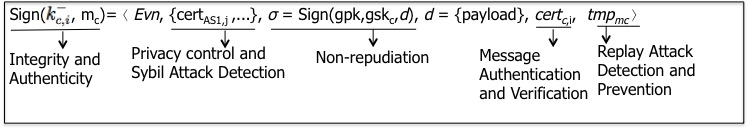
\includegraphics[scale=.43]{figures/message-format.jpg}
\caption{The format of beacon or event-driven messages and the field goals.}
\label{fig:msg-format}
\end{figure} 

The multiple-pseudonym approach proposed herein may use any of the pseudonym change approaches available in the literature~\cite{lu2012pseudonym}, \cite{mix-zone-vanets}, \cite{buttyan2007effectiveness}, \cite{caravan}, \cite{buttyan2009slow} and \cite{mix-zone-motion}. However, the change of pseudonyms may imply a change on the current anonymity set digital certificates $CERT^{t}_{AS_{c}}$ that the vehicle $v_{c}$ must use, as defined on the Property 3 (b) of the Multilevel \protocolname~Architecture. 

%For instance, suppose that $v_{c}$ belongs to the following anonymity sets of 5 levels ($m = 5$): $AS_{c} = \{AS_{1,1}, AS_{1,3}, AS_{1,12}, AS_{1,22}, AS_{1,35}, AS_{2,5}, AS_{2,9}, AS_{2,18}, \newline AS_{2,23}, AS_{3,6}, AS_{3,15}, AS_{3,21}, AS_{4,9}, AS_{4,27}, AS_{4,32}, AS_{5,2}, AS_{5,11}, AS_{5,23}, AS_{5,43}\}$. If $v_{c}$ is currently sending messages with pseudonym $cert_{c, 3} \in TK_{c}$  and its current anonymity set digital certificates is $CERT^{t_{1}}_{AS_{c}} = \{cert_{AS_{1, 3}}$, $cert_{AS_{2, 18}}$, $cert_{AS_{3, 6}}$, $cert_{AS_{4, 32}}$, $cert_{AS_{5, 23}}\}$, then the change from the pseudonym $cert_{c, 3}$ to $cert_{c, 4} \in TK_{c}$ requires a new subset $CERT^{t_{2}}_{AS_{c}}$ of anonymity set digital certificates. This approach aims to avoid pseudonym linkage, in which an eavesdropper is able to associate two or more pseudonyms that belong to the same vehicle in different time intervals. 

%For instance, suppose that two vehicles  $v_{A}$ and $v_{B}$ belong to the first level anonymity sets $AS_{1,2}$ and $AS_{1,3}$, respectively. Hence, their messages must include at least the digital certificates $cert_{AS_{1, 2}} \in CERT^{t1}_{AS_{A}}$ and $cert_{AS_{1, 3}} \in  CERT^{t1}_{AS_{B}}$, respectively. Now consider the following scenario depicted in Figure~\ref{fig:pseudonymchangeslink}: both vehicles form a mix zone and start a pseudonym change process at time $t_{1}$. If vehicle $v_{A}$ changes the pseudonym $cert_{A,1} \in TK_{A}$ to $cert_{A, 2} \in TK_{A}$, $v_{B}$ changes from $cert_{B, 1}  \in TK_{B}$ to $cert_{B, 2}  \in TK_{B}$, but they also keep their current anonymity set digital certificates as $cert_{AS_{1, 2}}$ and $cert_{AS_{1, 3}}$ at time $t_{2}$ (i.e.: $CERT^{t2}_{AS_{A}} = CERT^{t1}_{AS_{A}}$ and $CERT^{t2}_{AS_{B}} = CERT^{t1}_{AS_{B}}$), then an eavesdropper may link both changes by analyzing the first level anonymity set digital certificates (i.e.: $cert_{AS_{1, 2}}$ and $cert_{AS_{1, 3}}$). On the other hand, if both vehicles also change their current anonymity set digital certificates at time $t_{2}$ ($CERT^{t1}_{AS_{A}} \neq CERT^{t2}_{AS_{A}}$ and $CERT^{t1}_{AS_{B}} \neq CERT^{t2}_{AS_{B}}$), then it is difficult to link new and previous pseudonyms.
%
%\begin{figure}[ht]
%\centering
%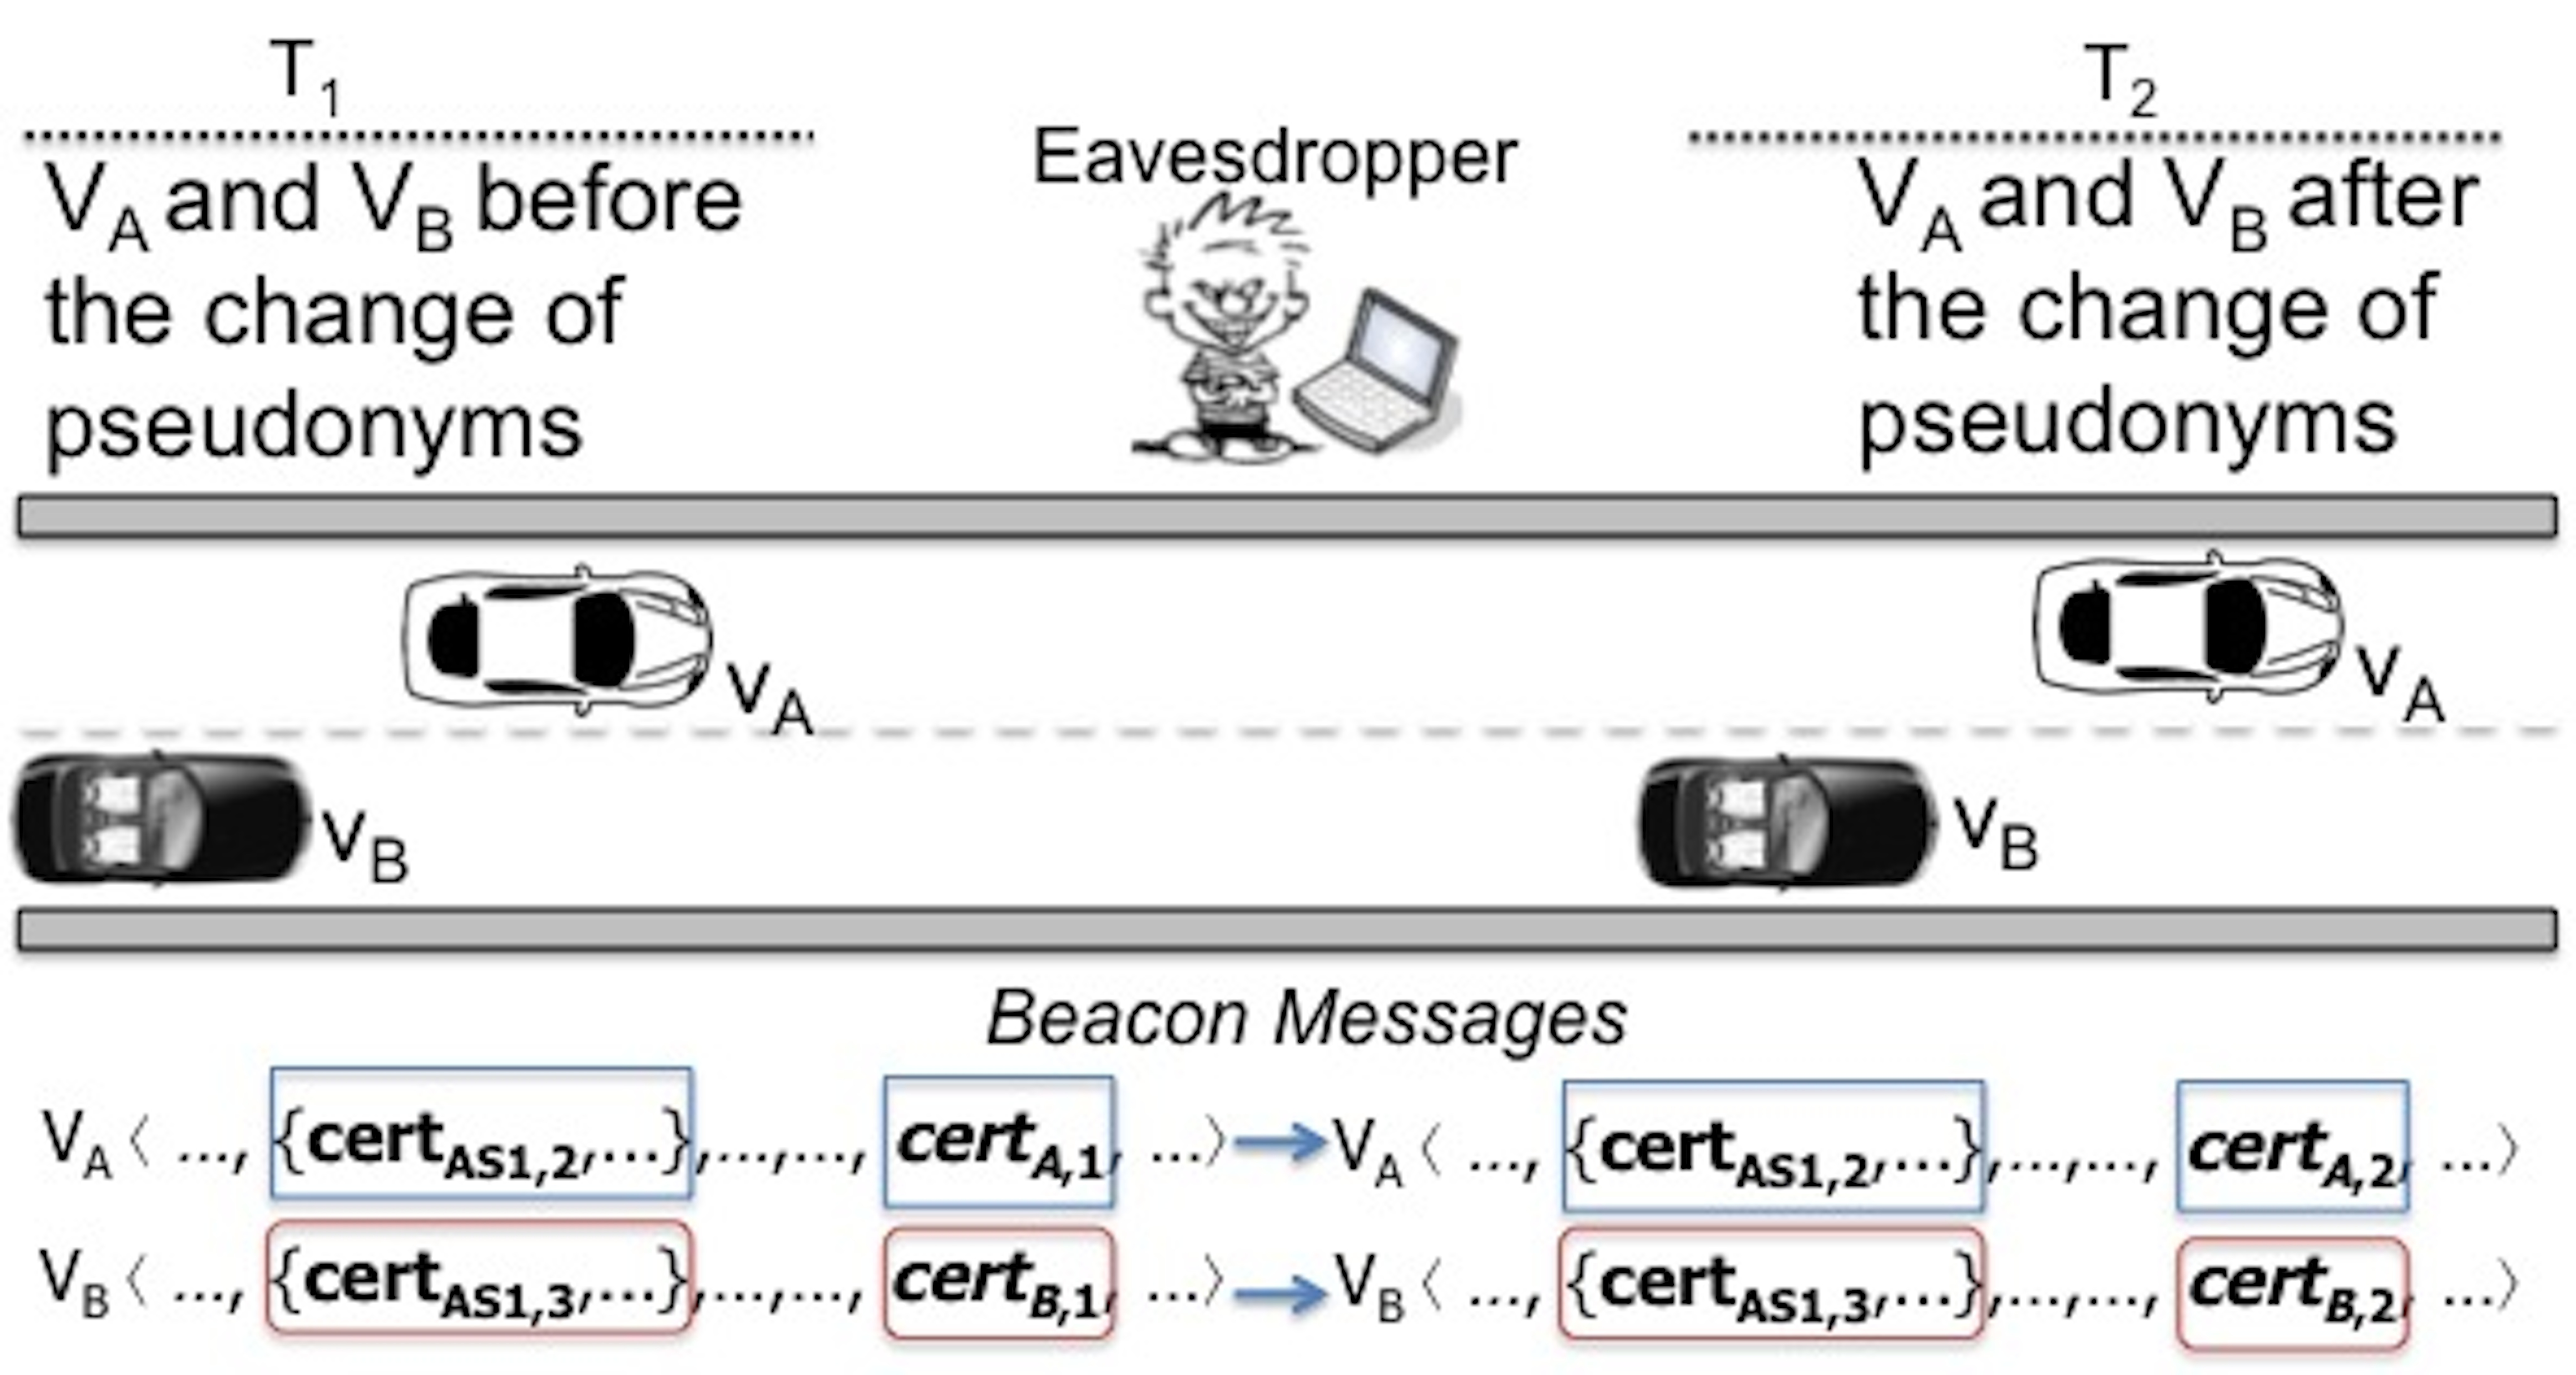
\includegraphics[scale=.53]{figures/cenario-mudanca-pseud-1-en.jpg}
%\caption{An eavesdropper may link old and new pseudonyms if vehicles do not change their current anonymity set digital certificates during the change of pseudonyms.}
%\label{fig:pseudonymchangeslink}
%\end{figure} 

The TPD will not change the current subset from $CERT^{t}_{AS_{c}}$ to $CERT^{t+1}_{AS_{c}}$ if the last change occurred in a time less than $\tau$ units of time. This decision helps to avoid \textit{sybil} attacks, which comprise the third phase of the \protocolname~protocol and is discussed on the next section.

When a vehicle $v_a$ receives a message $m_c$ from a vehicle $v_c$, it needs to verify $m_c$ in two steps: first, the $v_c$'s $cert_{c,i}$ authenticity; and second, if $m_c$ is a new message (not originated from a replay attack). In the former case,  $cert_{c,i}$ is authentic if, and only if, $cert_{c,i}$ was digitally signed from an RSU, as well as $cert_{c,i}$ is still valid regarding its lifetime. In the second case, $m_c$ is valid if, and only if, $v_c$ signed $m_c$ and if $m_c$ has been uttered only recently.


%, which is detailed in Equation~\ref{eq:verifica-autenticidade-certificado-temporario}.
%
%
%\begin{equation}
%	\label{eq:verifica-autenticidade-certificado-temporario}
%		Verify(k^{+}_{RSU}, cert_{c, i}) = valid \leftrightarrow Signed^{cert_{c,i}}_{RSU} \wedge (tmp - tmp_{cert_{c,i}} \le threshold_{max})
%\end{equation}
	
%, which is detailed in Equation~\ref{eq:verifica-autenticidade-mensagem}.
%
%\begin{equation}
%	\label{eq:verifica-autenticidade-mensagem}
%		Verify(k^{+}_{c, i}, m_{c}) = valid \leftrightarrow Signed^{m_{c}}_{v_{c}} \wedge (\textit{tmp} - tmp_{m_{c}} \le threshold_{max})
%	\end{equation}

\subsection{The \textit{Sybil} Attack Detection (Phase 3)}
\label{sec:sybildetec}

The third phase of the \protocolname~protocol is the \textit{sybil} attack detection itself. A \textit{sybil} attack may be explored from malicious users that modify their vehicles to launch the attack. The \textit{sybil} attack is defined as follows:

%In short, to detect a \textit{sybil} node while keeping vehicles' privacy, consider that any vehicle will send messages with a subset of anonymity set digital certificates. In a given time interval \textit{t}, a legitimate vehicle sends messages with one pseudonym that carries a subset of anonymity set digital certificates. 
%However
%\textit{Sybil} nodes send messages with multiple pseudonyms (at the same time) with the same subset of anonymity set digital certificates. Therefore, if a vehicle receives messages with different pseudonyms, but with the same subset of anonymity set digital certificates, then, the receiver detected a \textit{sybil} attack. 

%After detecting a \textit{sybil} node, the Certificate Authority may identify the malicious vehicle through the group signatures (which comprises the fourth phase of ASAP-V).

\begin{definition}
\label{def:sybil-event}
In the sybil attack, a vehicle uses multiple identities to disseminate the same false event. This vehicle is the sybil vehicle.
\end{definition}

In VANETs, vehicles disseminate events in order to provide vehicular safety applications. Examples may include accident reporting, an approaching safety vehicle, and electronic emergency braking warnings, to name a few. These events are classified as sporadic events. Beacon messages, may also be an event and are classified as periodic events. An event is defined as follows:

\begin{definition}
\label{def:event}
An event, as defined in~\cite{p2dap2}, is represented as a tuple $\langle evt, l, t \rangle$, where \textit{evt} is the event type, \textit{l} and \textit{t} are the location and the time interval in which the event occurred, respectively.
\end{definition}

The privacy-preserving \textit{sybil} detection phase explores the multilevel anonymity set architecture to detect \textit{sybil} attacks from beacon and event-driven messages. The properties 1 to 3 provide privacy control, while property 4 allows the \textit{sybil} detection process. The basic detection concept is as follows: any two or more messages with different pseudonyms, which disseminate the same event, cannot include the same subset of anonymity set digital certificates. Hence, during a \textit{sybil} attack, the system must evaluate the Equation~\ref{eq:sybil-detection-eq}, where $V_{l}$ is the set of vehicles in the transmission range in a given location \textit{l}.  

\begin{equation}
\label{eq:sybil-detection-eq}
\forall (v_{c}, v_{c'}) \in V_{l} (\thinspace |CERT^{t}_{AS_{c}}| = |CERT^{t}_{AS_{c'}}| \wedge CERT^{t}_{AS_{c}} - CERT^{t}_{AS_{c'}} \neq \emptyset)
\end{equation}

In beaconing-like messages, if any vehicle $v_{b}$ receives beacon messages from vehicle $v_{a}$, ($v_{a}, v_{b}) \in V_{l}$, and these messages include the same subset $CERT^{t}_{AS_{b}}$ of $v_{b}$' anonymity set digital certificates, then both vehicles gradually attach, into their beacon messages, the digital certificate of the next deeper anonymity set until the Equation~\ref{eq:sybil-detection-eq} is satisfied, where all messages are distinguishable among each other.

%For instance, consider the scenario depicted in Figure~\ref{fig:sybil2}. The malicious vehicle $v_{e}$ (\textit{sybil}) and the legitimate one $v_{a}$ are, among \textit{k} anonymity sets per level, in the following anonymity sets for 5 levels ($m = 5$), respectively: $AS_{e}$ = \{$AS_{1,2}$, $AS_{2,4}$, $AS_{3,2}$, $AS_{4,6}$, $AS_{5,1}$\}, $AS_{a}$ = \{$AS_{1,2}$, $AS_{2,4}$, $AS_{3,2}$, $AS_{4,4}$, $AS_{5,2}$\}. Each vehicle also stores its current anonymity set digital certificates as $CERT^{t}_{AS_{e}}$ = \{$cert_{AS_{1,2}}$, $cert_{AS_{2,4}}$, $cert_{AS_{3,2}}$, $cert_{AS_{4,6}}$, $cert_{AS_{5,1}}$\}, $CERT^{t}_{AS_{a}}$ = \{$cert_{AS_{1,2}}$,  $cert_{AS_{2,4}}$, $cert_{AS_{3,2}}$, $cert_{AS_{4,4}}$, $cert_{AS_{5,2}}$\}. Furthermore, suppose that the vehicles also store \textit{w} temporary key pairs $TK_{e}$ and $TK_{a}$.

%\begin{figure}[h]
%\centering
%\caption{Detecting \textit{sybil} attacks from beacon messages.}
%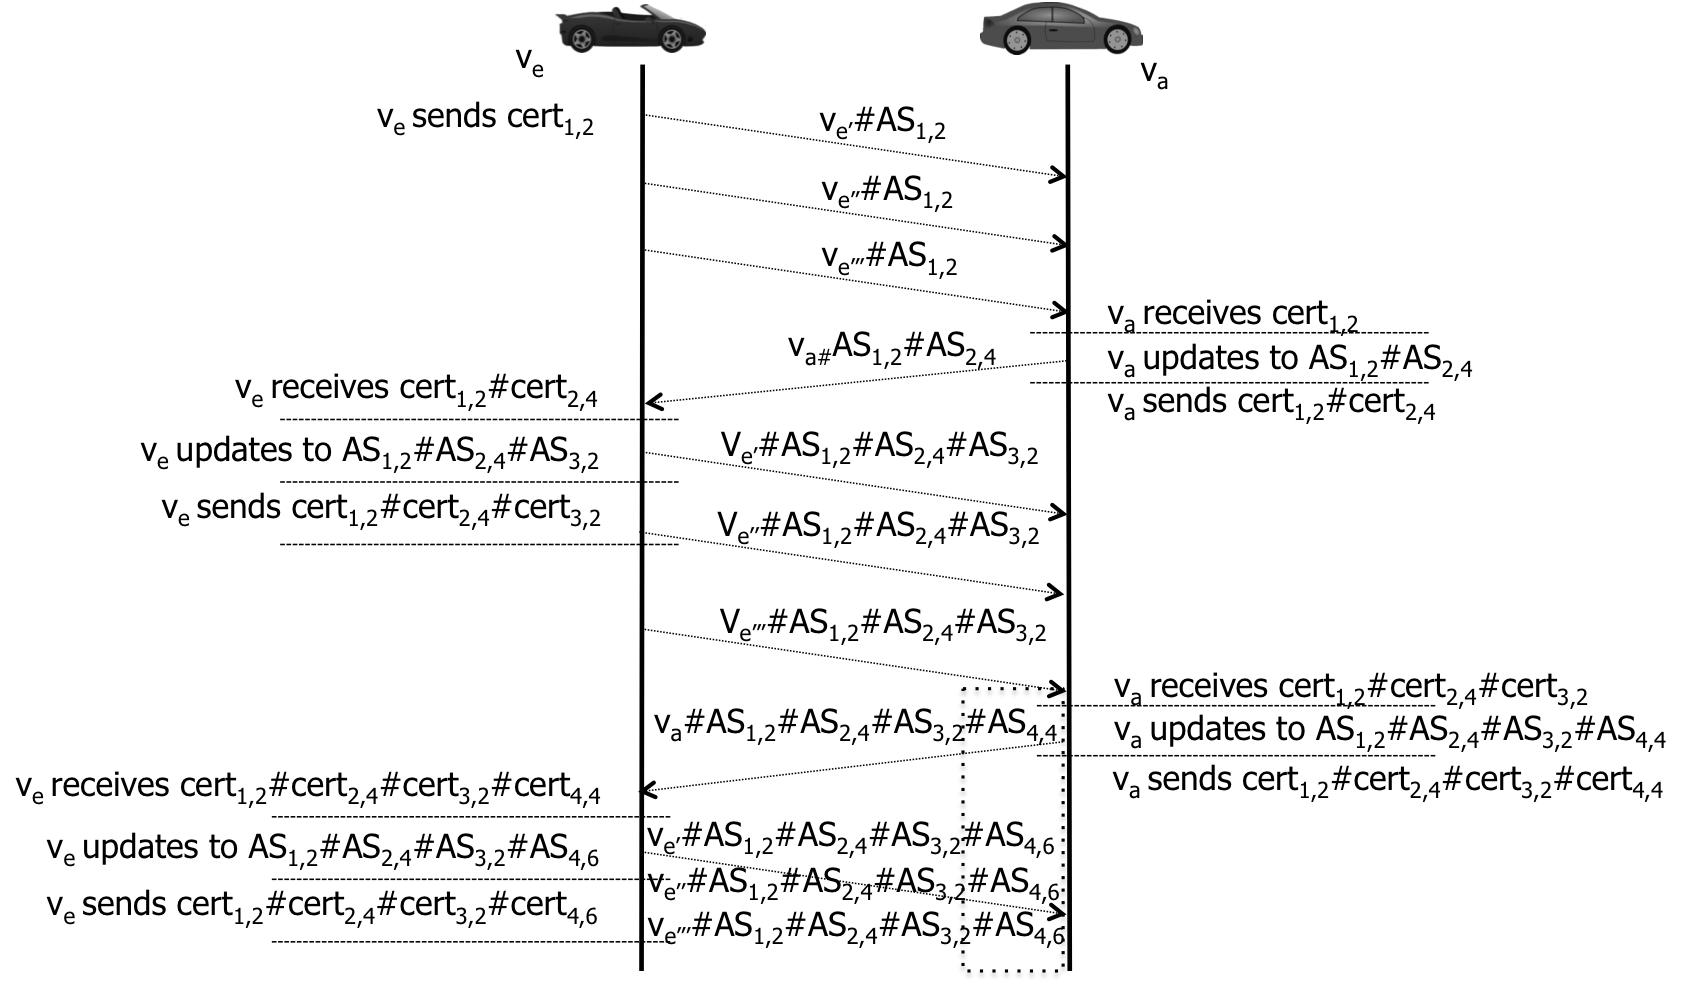
\includegraphics[scale=0.6]{figures/cenario-sybil-5-execution-en.png}
%\label{fig:sybildetectionexecution}
%\end{figure}

\begin{figure}[h]
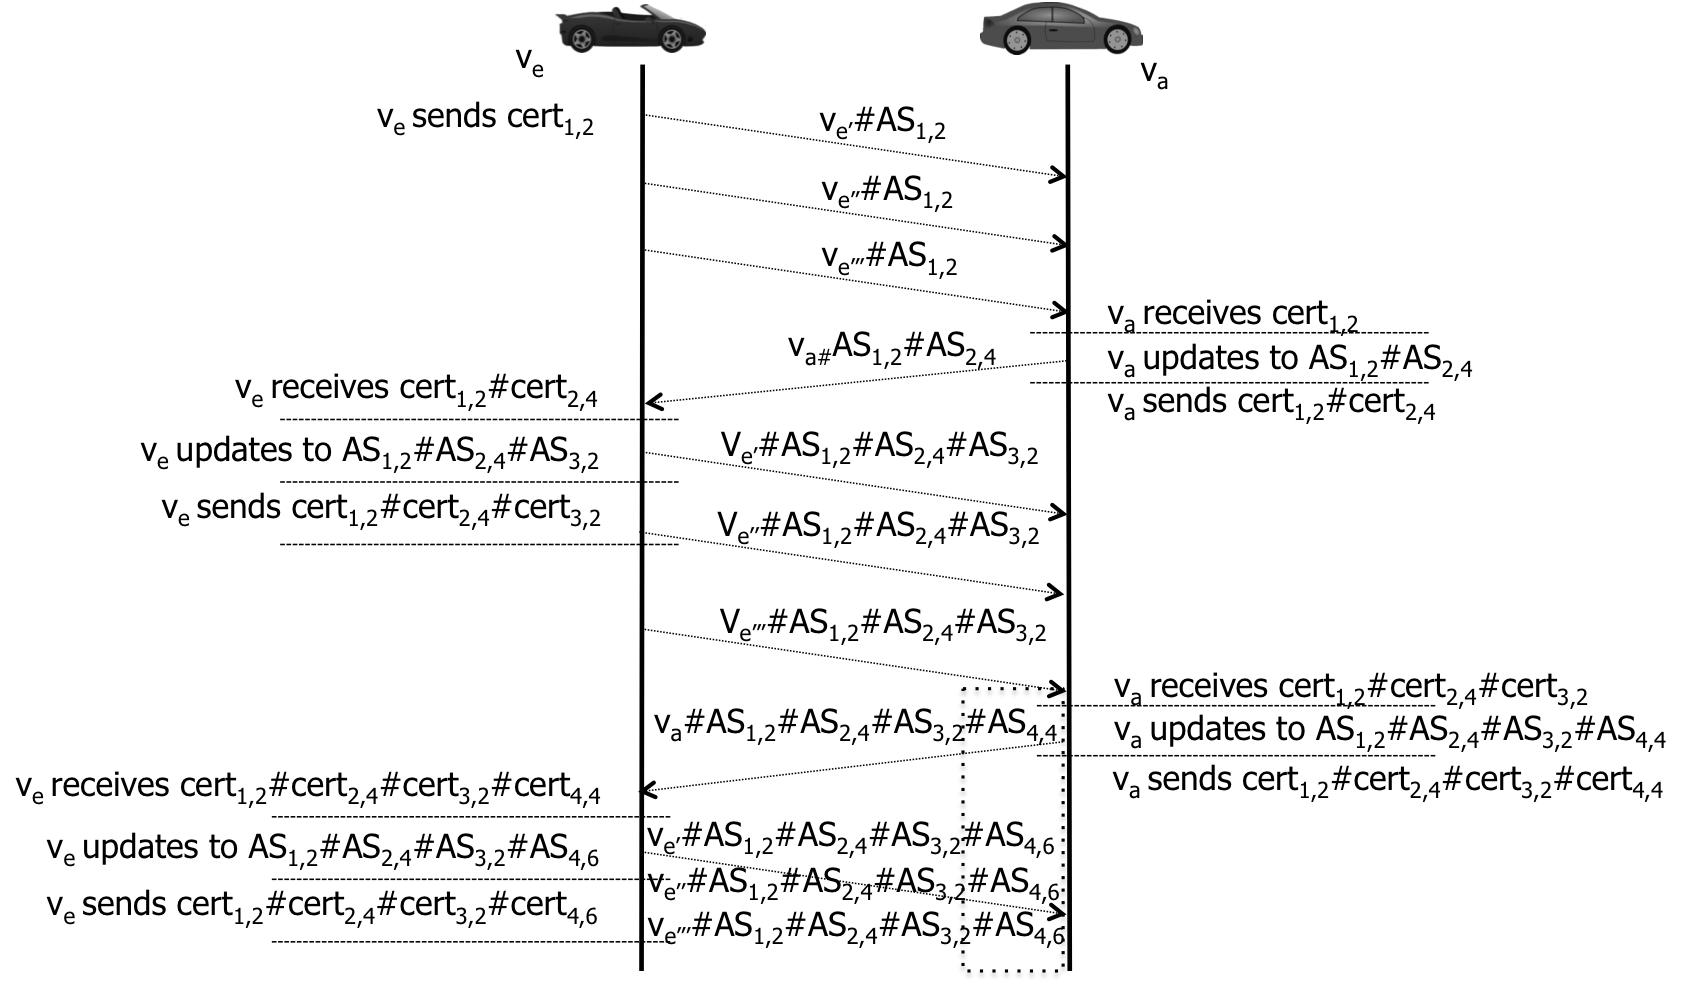
\includegraphics[width=4.5in]{figures/cenario-sybil-5-execution-en.png}
\caption{
Detecting \textit{sybil} attacks from beacon messages. To detect a \textit{sybil} attack, messages with different pseudonyms carry the same subset of anonymity set digital certificate.}
\label{fig:sybildetectionexecution}
\end{figure}

Figure~\ref{fig:sybildetectionexecution} depicts the \textit{sybil} attack detection. The malicious vehicle $v_{e}$ fires a \textit{sybil} attack by sending 3 different beacon messages that describe 3 location points. Since beacon messages are broadcasted to all vehicles in the transmission range, the vehicle $v_{a}$ observes that other vehicle(s) is (are) transmitting messages that contain the same first level anonymity set digital certificate ($AS_{1, 2}$). $v_{a}$ attaches the next anonymity set digital certificate (e.g.: $cert_{2,4}$) and sends it on its next beacon message. 

When $v_{e}$ receives $v_{a}$'s message, it must have to update to the next two levels. Since $v_{e}$ knows that it also belongs to anonymity set $AS_{2, 4}$, it also must include the third anonymity set digital certificate (e.g.; $cert_{3, 2}$), otherwise vehicles in the vicinity will only drop the messages and the \textit{sybil} attack has no effect. On the other hand, the other vehicles (e.g.: $v_{b}$, $v_{c}$, $v_{d}$, $v_{f}$, $v_{g}$) only store $v_{e}$'s and $v_{a}$'s messages. After receiving $v_{e}$'s messages, $v_{a}$ attaches the fourth level anonymity set digital certificate (e.g.: $cert_{4, 4}$) and sends it all together. Finally, the malicious vehicle sends its fourth level anonymity set digital certificate (e.g.: $cert_{4,6}$). 

Note that if a malicious vehicle $v_{e}$ sends messages with multiple identities, these messages will always carry the same set of anonymity set digital certificates. That is, only messages from identities $v_{e'}$, $v_{e''}$ and $v_{e'''}$ do not satisfy Equation~\ref{eq:sybil-detection-eq}. Therefore, vehicles $v_{a}$, $v_{b}$, $v_{c}$, $v_{d}$, $v_{g}$ and $v_{f}$ store the messages from $v_{e}$ as a set of \textit{n} messages $M_{e, n}$, which is used for prosecution purpose (Phase 4, detailed in Section~\ref{sec:phase4}).

After a short time interval receiving messages with different identities, but still containing the same anonymity set digital certificates, the legitimate vehicles may conclude that the messages with these identities come from a \textit{sybil} node (e.g.: $v_{e}$). Equation~\ref{eq:wait-time} defines this short time interval that the vehicles $v_{a}$, $v_{b}$, $v_{c}$, $v_{d}$, $v_{g}$ and $v_{f}$ must wait for vehicle $v_{e}$ to send the next anonymity set digital certificate after receiving the last one. 

The time interval is evaluated for each group of messages that contain the $AS_{1, j}$'s anonymity set digital certificate. The \textit{m} variable is the maximum number of anonymity set levels, \textit{pm} is the number of anonymity set digital certificates already presented by the target vehicle, and $V_{l}$ is the number of neighboring nodes in the transmission range. Therefore, after $\delta_{AS_{1,j}}$ \textit{ms} after receiving the last anonymity set digital certificate, the vehicles $v_{a}$, $v_{b}$, $v_{c}$, $v_{d}$, $v_{g}$ and $v_{f}$ may evaluate the vehicle $v_{e}$ as a \textit{sybil} node.

\begin{equation} 
\label{eq:wait-time}
\delta_{AS_{1,j}}  = \textit{\text{beacon interval}} + (m - pm) * V_{l} / m
\end{equation}

Equation~\ref{eq:wait-time} defines a dynamic behavior in which $\delta_{AS_{1,j}}$ must be as high as the number of vehicles in the transmission range is high, but, in order to minimize the impact of the \textit{sybil} attack, $\delta_{AS_{1,j}}$ smoothly decreases as the number of presented anonymity set digital certificates per level within the beacon messages increases. A vehicle evaluates Equation~\ref{eq:wait-time} for each new beacon message that it receives and contains the anonymity set digital certificate $cert_{AS_{1, j}}$. If a malicious vehicle try to evade the \textit{sybil} attack after it had been fired and before achieving the last level of possible anonymity sets, then the $\delta_{AS_{1,j}}$ time interval will timeout and the sample suspected messages will be used in the prosecution phase.

%the scenario depicted in Figure~\ref{fig:false-positive-result-scenario}. It is 

%Now, consider a classical hidden terminal scenario (caused by fading) where tow vehicles, \textit{C} and \textit{A}, belong to the same first level anonymity set (e.g.: $AS_{1,2}$). Another vehicle \textit{B} receives beacon messages from the vehicles \textit{C} and \textit{A}. However, due to the \textit{A}'s and \textit{C}'s transmission ranges, neither \textit{A} nor \textit{C} receive the messages from each other. Therefore, they keep sending messages with their first level anonymity set digital certificate $cert_{AS_{1,2}}$. From the \textit{B}'s perspective, since the vehicles \textit{A} and \textit{C} keep sending messages without presenting the next anonymity set digital certificates, after $\delta$ \textit{ms} (Equation~\ref{eq:wait-time}), \textit{B} evaluates \textit{A}'s and \textit{C}'s messages as originated from a \textit{sybil} vehicle. However, both A and C are two benign vehicles.

%\begin{figure}[ht]
%\centering
%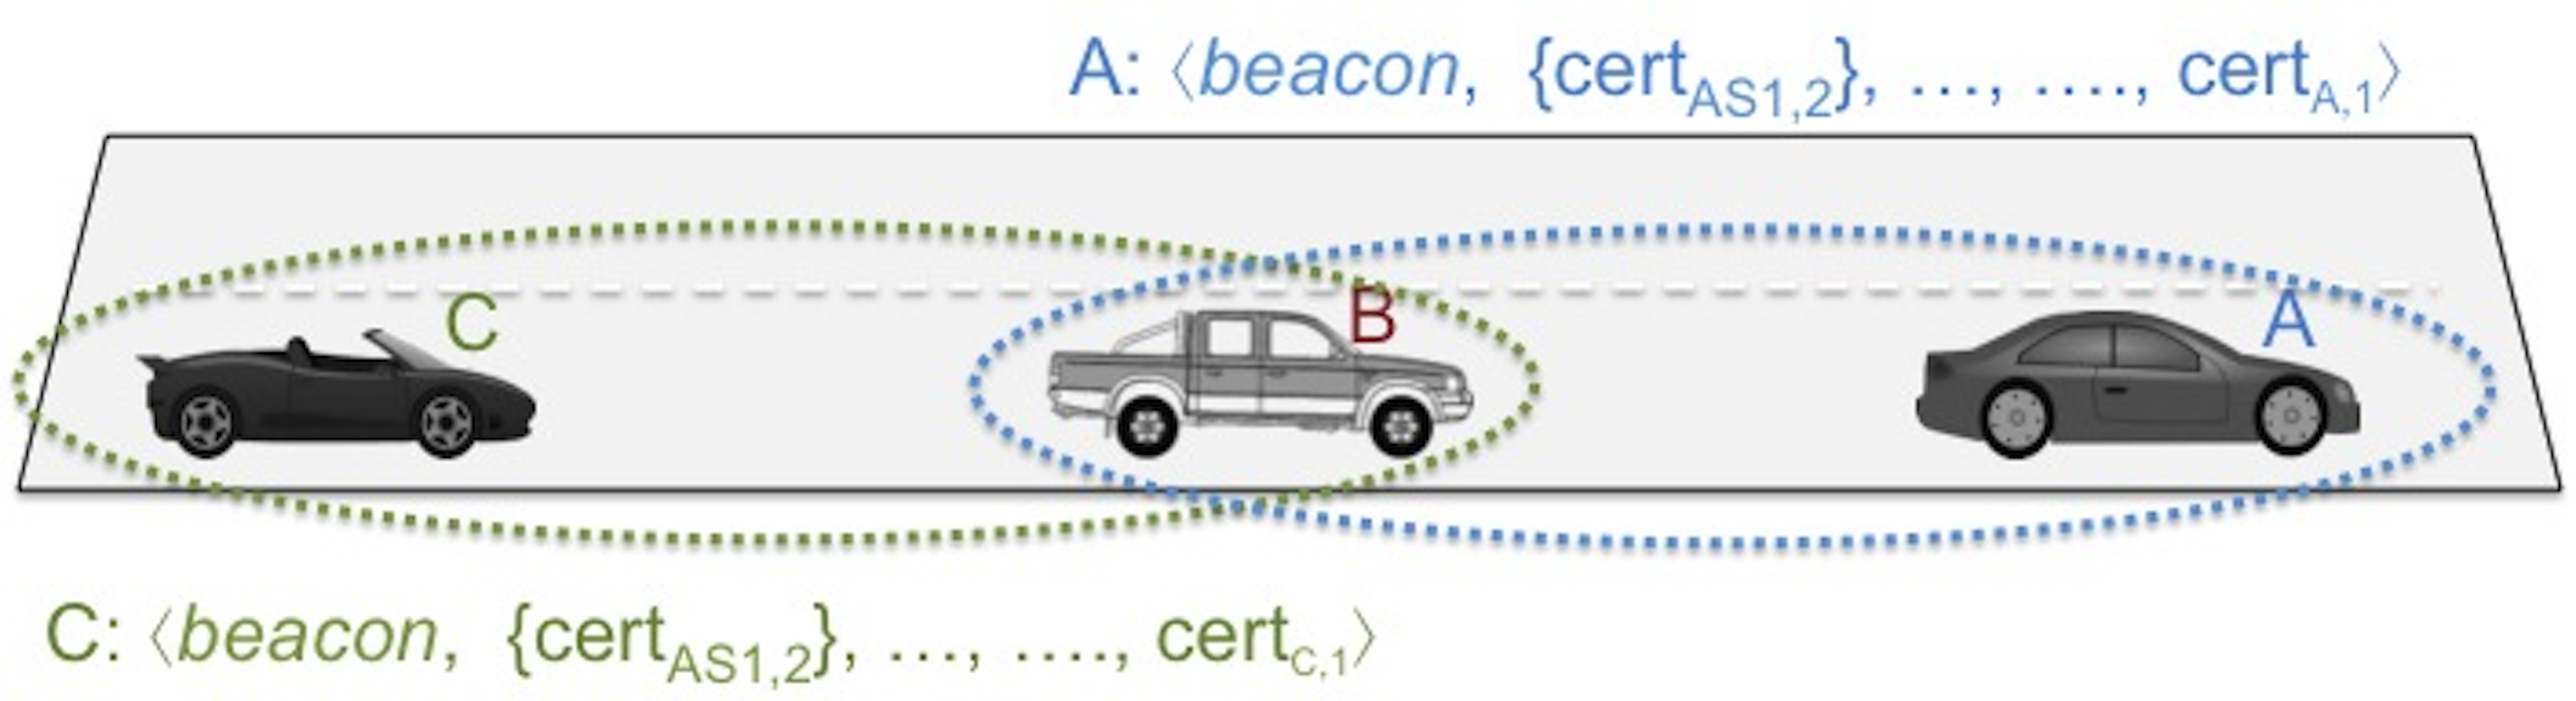
\includegraphics[scale=.45]{figures/false-positive-scenario.jpg}
%\caption{Hidden terminals scenarios may lead to false-positive \textit{sybil} detections.}
%\label{fig:false-positive-result-scenario}
%\end{figure}

On the other hand, hidden terminal scenarios (caused by fading) may lead to false-negative \textit{sybil} detections. To avoid hidden terminals in \protocolname~protocol, we propose the \textit{sybil attack signaling message}, which we also call as \textit{First Level Warning} (FLW) message. It aims at allowing one vehicle to announce to neighboring vehicles that there are two or more vehicles in the vicinity that belong to the same first level anonymity set. This signaling message aims to avoid \textit{false-positive} detections in hidden terminals scenarios. For instance, as depicted in Figure~\ref{fig:first-level-signaling-message}, vehicle B ($v_b$) broadcasts signaling messages with identities A and C. Once all vehicles may listen to the \textit{signaling} messages in the broadcast channel, the vehicles A and C may detect that they are suspected and may attach the next anonymity set digital certificates in their next beacon messages.

\begin{figure}[ht]
\centering
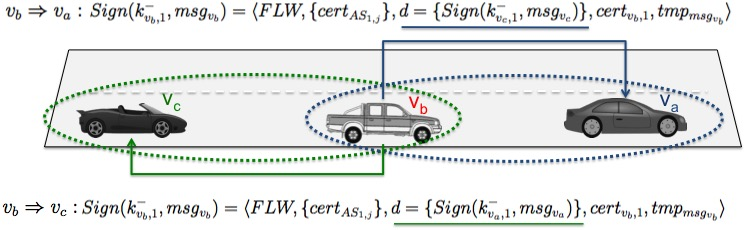
\includegraphics[scale=.38]{figures/signiling-message-scenario.jpg}
\caption{Vehicle $v_{b}$ sends FLW message as \textit{signaling message} to vehicles $v_{a}$ e $v_{c}$.}
\label{fig:first-level-signaling-message}
\end{figure}

To detect if two vehicles $v_a$ and $v_c$ are hidden terminals to each other, one vehicle (e.g: $v_b$) must evaluate if their transmission signals do not reach the other one. Let $P_{x, pos_y}$ be the power of the transmission signal of vehicle $v_x$ at position \textit{y}. Thus, we must evaluate if $P_{a, pos_c} < P_{min}$ and $P_{c, pos_a} < P_{min}$, where $P_{min}$ is the minimum power required to receive a beacon message successfully.

To evaluate $P_{a, pos_c}$ and $P_{c, pos_a}$, we first need to estimate the initial power of the signals transmitted from $v_a$ and $v_c$, that is, $P_{a, pos_a}$ and $P_{c, pos_c}$. Let $\alpha$ be a constant associated to the exponential decay of the power of the electromagnetic wave as the signal travels along the communication channel in a dissipative dielectric, and $d(_{v_x, v_y})$ the euclidean distance between vehicles $v_x$ and $v_y$.

%$P_{a, pos_b}$ and $P_{c, pos_b}$ be the power of the transmission signals of vehicles $v_a$ and $v_c$ at $v_b$'s current position, respectively. 

%b => c, a => b
%P_{c, pos_b} & = P_{c, pos_c}\cdot e^{- \alpha \cdot d(_{v_c, v_b})}
%P_{c, pos_c} & = P_{c, pos_b}\cdot e^{\alpha \cdot d(_{v_c, v_b})}
%

\begin{align*} 
  P_{a, pos_b} & = P_{a, pos_a}\cdot e^{- \alpha \cdot d(_{v_a, v_b})}\tag{The transmitted signal power of $v_a$ at $v_b$'s position.}\\
  P_{a, pos_a} & = P_{a, pos_b}\cdot e^{\alpha \cdot d(_{v_a, v_b})}\tag{(2) The initial transmitted signal power of $v_{a}$} 
\end{align*}
\begin{align*} 
  P_{c, pos_b} & = P_{c, pos_c}\cdot e^{- \alpha \cdot d(_{v_c, v_b})}\tag{The transmitted signal power of $v_c$ at $v_b$'s position}\\
  P_{c, pos_c} & = P_{c, pos_b}\cdot e^{\alpha \cdot d(_{v_c, v_b})}\tag{(1) The initial transmitted signal power of $v_{c}$} 
\end{align*}
\begin{align*}
  P_{a, pos_c} & = P_{a, pos_a}\cdot e^{- \alpha \cdot d(_{v_a, v_c})}\\\tag{(3) The transmitted signal power of $v_a$ at $v_c$'s position}
\end{align*}
\begin{align*}
  P_{c, pos_a} & = P_{c, pos_c}\cdot e^{- \alpha \cdot d(_{v_c, v_a})}\\\tag{(4) The transmitted signal power of $v_c$ at $v_a$'s position}
\end{align*}

Therefore, applying (1) to (3) and (2) to (4), the transmitted signal power of $v_a$ at $v_c$'s position, and the $v_c$ at $v_a$'s position are defined in Equations~\ref{eq:estimatepower1} and \ref{eq:estimatepower2}, respectively:

\begin{equation} 
\label{eq:estimatepower1}
\begin{split}
P_{a, pos_c} & = P_{a, pos_b}\cdot e^{\alpha \cdot d(_{v_a, v_b})} \cdot e^{- \alpha \cdot d(_{v_a, v_c})}
\end{split}
\end{equation}
\begin{equation} 
\label{eq:estimatepower2}
\begin{split}
P_{c, pos_a} & = P_{c, pos_b}\cdot e^{\alpha \cdot d(_{v_c, v_b})} \cdot e^{- \alpha \cdot d(_{v_c, v_a})}
\end{split}
\end{equation}

Thus, if $P_{a, pos_c} < P_{min}$ and $P_{c, pos_a} < P_{min}$, vehicle $v_b$ must send FLW messages to vehicles $v_a$ and $v_c$. Hence, both vehicles may attach their next anonymity set digital certificates. Since FLW messages are sent in a broadcast manner, all other vehicles in the vicinity will also receive $v_b$'s FLW message. This approach avoids multiple FLW messages to the same scenario.

In order to detect \textit{sybil} attacks from event-driven messages, each vehicle $v_{i}$ must attach all current anonymity set digital certificates ($CERT^{t}_{AS_{i}}$) in the message. Suppose the vehicle $v_{a}$ reports an emergency braking alert (EBBL). Hence, the messages would be as follows:  $Sign(k^{-}_{a,1}, m_a)$ = $\langle $EBBL, ($\boldsymbol{cert_{AS_{1,2}}}$, $\boldsymbol{cert_{AS_{2,4}}}$, $\boldsymbol{cert_{AS_{3,2}}}$, $\boldsymbol{cert_{AS_{4,4}}}$, $\boldsymbol{cert_{AS_{5,1}}}$), $\sigma = Sign(gpk, gsk_{a}, d)$, $d = ....., cert_{a, 1}, tmp_{m_a} \rangle$. According to property 4 of the multilevel anonymity sets architecture, it is impossible for two different vehicles to announce the same event with the same \textit{anonymity set digital certificates}. This approach definitely avoids a \textit{sybil} attack from event-driven messages without compromising the privacy of the vehicles.

\subsection{Sybil Attack Prosecution Phase (Phase 4)}
\label{sec:phase4}

Once a misbehaved vehicle $v_{e}$ is detected, all other vehicles $v_{i}$ in \textit{l} store $v_{e}$'s messages as a set of sample \textit{n} suspected messages $M_{e, n}$. Thus, a prosecution protocol is executed. 

In Step 1, each vehicle $v_{i}$ generates a digitally signed prosecution message and sends it to the nearby RSU. Each vehicle $v_{i}$ that detected the \textit{sybil} vehicle (e.g.: $v_{a}$ and $v_{b}$) uses it's group signing key (e.g.: $gsk_{a}$ and $gsk_{b}$) to digitally sign the prosecution message, and also attach the sample of suspected messages evaluated as \textit{sybil} messages (e.g.: $m_{e, 1}$, $m_{e, 2}$, $m_{e, 3}, ..., m_{e, n} \in M_{v_{e}, n}$). In Step 2, the RSU forwards the received prosecution messages to the CA. In Step 3, the CA extracts the suspected messages from the prosecution message and traces their owners using its \textit{gmsk} key. If all \textit{n} messages describe the same event \textit{evt} and are originated from the same vehicle $v_{e}$ (it digitally signed all messages), then the CA resolves each message to the same unique vehicle identity (i.e.: a \textit{sybil} vehicle). Equation~\ref{eq:traceall} formally describes the verification process. Finally, the CA inserts the malicious vehicle's group revocation token (e.g.: $grt_{e}$) into the revocation token list (RL), and sends the RL to all RSUs in Step 4. 
%
%\begin{figure}[ht]
%\centering
%\includegraphics[scale=.4]{figures/acusacao-en.jpg}
%\caption{The prosecution of misbehaved vehicles.}
%\label{fig:accusation}
%\end{figure}

\begin{equation} 
\label{eq:traceall}
\begin{split}
TraceAll(gmsk, M_{v_{e}, n}) = \forall m_{i}, m_{j} \in M_{v_{e},n}, (evt_{i} \in m_{i} = evt_{j} \in m_{j}) \wedge \\ 
(Signed^{\sigma_{i}}_{v_{e}} \wedge Signed^{\sigma_{j}}_{v_{e}}) \leftrightarrow sybil_{v_{e}} \{i, j, n \in \mathbb{N} : 1 \le i \le n, 1 \le j \le n, i \neq j\}
\end{split}
\end{equation}

\section{Protocol Analysis and Experimental Results}
\label{sec:results}

This section presents the experimental results of the proposed solution. First, we analyze the management, storage, computation, and communication overheads; mainly w.r.t. the cryptography key management and its processing. Afterwards, we show the correctness verification of the pseudonym renewal protocol, as well as an analysis of the proposed anonymous communication model. Finally, we present the simulation results of the proposed \textit{sybil} detection approach. 

\subsection{Management, Storage, Computation and Communication Overheads}
\label{sec:overheads}
In spite of the number of security properties involved, the following overhead analysis shows that \protocolname~is a lightweight protocol within the context of VANETs.

\begin{itemize}
	\item \textit{Management overhead}: the CA is only responsible for managing the anonymity set digital certificates and the group signing keys, which do not change frequently. In addition, vehicles must only manage the pseudonyms renewal that requires minimal changes;

	\item \textit{Storage overhead}: the CA stores the anonymity set digital certificates, which takes $n*m*56$ bytes long using a 224bits Elliptic Curve Digital Signature Algorithm (ECDSA)~\cite{elliptic-curve}, the group public key with size $O(log\thinspace |V|)$, which takes $|V| * 800$ bytes long, and the group membership certificate of size $O (1)$, which takes $|V|*64$ bytes long using Group Signatures with Almost-for-free Revocation (GSAFR)~\cite{libert2012group}. It is important to note that the CA does not need to store vehicle pseudonyms, which reduces the storage overhead found in other works, such as the Zhou's approach~\cite{p2dap2} and \cite{p2dap}. Moreover, the RSUs store the Revocation List of size \textit{O(log r)} (which contains each vehicle's group revocation tokens), which is also small when compared with traditional revocation lists of the public key infrastructure (which stores all non-valid public keys). 
	
	%Finally, vehicles store only the set of \textit{w} pseudonyms (public/private key pairs and digital certificates), which are \textit{w}*56 bytes long, as well as the anonymity set digital certificates, which are $k*m*56$ bytes long, and the public and private group signing keys, which are 800 and 64 bytes long;
	
	%NO NOSSO EXEMPLO ANTERIOR, CADA VEICULO ARMAZENARIA 6720 BYTES - 6,5 MB ou 7,4 (com grupo)
	
	\item \textit{Computation Overhead}: we implemented our security algorithms on a 2.9 GHz Intel Core i7 processor with 8 GB of RAM, for V2V and V2I communications:
	
	\begin{itemize}
		\item On V2V communication: to sign a message in a V2V communication, a vehicle $v_{c}$ first signs the payload \textit{d} ($\sigma$) with its group signing key $gsk_{c}$ using GSAFR, which takes $11$ \textit{ms} with computation and size of cost $O (1)$; and afterwards, the whole message with its $i^{th}$ temporary private key $k^{-}_{c, i}$, which takes $0.1$ \textit{ms} using ECDSA. Thus, $v_{c}$ takes $11.1$ \textit{ms} to sign the whole message. On the other hand, when another vehicle $v_{e}$ receives the message, it verifies the message's authentication in two steps: first it verifies the sender's ($v_{c}$) public key $k^{+}_{c, i}$ authenticity, which is  available in the digital certificate $cert_{c, i}$; and second, the whole message authentication itself. Thus, a vehicle must first check the $cert_{c, i}$ authentication using the RSU's public key $k^{+}_{RSU}$, which takes $0.4$ \textit{ms}, and then the whole message's authentication, which also takes $0.4$ \textit{ms}. The total message verification process takes $0.8$ \textit{ms}. In short, a vehicle may sign $90$ messages/s, while it may verify 1250 messages/s (or 2500 messages/s after checking the first time).
		
%		It is important to point out that a vehicle does not need to check $cert_{c, i}$ of the subsequent messages nor each anonymity set digital certificates $cert_{AS_{i, j}}$, since the whole message authentication guarantees that the message is from a trusted TPD. Furthermore, $v_{e}$ does not need to check the group digital signature $\sigma$ since it is used mainly for non-repudiation purposes. 
			
		\item On V2I communication: a vehicle signs the payload data (UUID and the $v_{c}$'s $i^{th}$ digital certificate) with its group signing key, which takes 16 ms (with computation cost of $O (log\thinspace 1)$), and the request message $m_c$ with ECDSA, which takes 1 ms  (Step 1); when a RSU receives the message $m_c$ (Step 2), it checks the group signature authentication in 132 \textit{ms}, with computation cost of $O (1)$, while it generates each \textit{w} key pair in \textit{w}*83 \textit{ms}, and signs \textit{w} key pairs that takes \textit{w}*1 \textit{ms}. Hence, the total computation cost is 132 \textit{ms} + \textit{w}*83 \textit{ms} +  \textit{w}*1 \textit{ms}. 
		
		%In order to avoid high overhead during key generation, the RSU may generate the set of key pairs previously without waiting for vehicles' pseudonym renewal requests, which reduces $w*83 + w*1$ \textit{ms} in the computation cost.
	\end{itemize}
	
	\item \textit{Communication Overhead}:
	\begin{itemize}
		\item On V2V communication: the beacon message size basically requires one anonymity set digital certificate $cert_{AS_{1,j}}$, which takes 56 bytes in a 224\textit{bit} ECDSA; the group signature $\sigma$ of the payload \textit{d}, which takes 225 bytes (128 bits security level) with signature size of $O (1)$; the $i^{th}$ temporary digital certificate $cert_{v, i}$, which takes 56 bytes; and finally, the whole message authentication, which also takes 56 bytes. The minimum message size to be transmitted is 393 bytes. On the other hand, as the number of anonymity set digital certificates increases due to the \textit{sybil} detection phase, the message size is 56 bytes longer. 
		
		%Therefore, Table~\ref{tab:beacontransfertime} summarizes the beacon transfer times (in \textit{milliseconds}) for different WAVE data rates and message sizes (in bytes) as the number of anonymity set levels increases. These results  show that \protocolname~has low communication overhead. In the next subsection, we evaluate the \textit{sybil} detection process for Levels 4, 5 and 6;
%		
%		\begin{table}[ht]
%\caption{Beacon transfer times (\textit{ms}) for different message sizes (bytes) and data rates (Mbps).}
%{\small
%\hfill{}
%\begin{tabular}{l|cccccccc}
%\hline
%& \multicolumn{8}{c}{Data rates (Mbps) in VANET.}                 \\ \hline
%\begin{tabular}[c]{@{}l@{}}Message Size \end{tabular} & 3    & 4.5  & 6    & 9    & 12   & 18   & 24   & 27    \\\hline
%393                                                             & 1.04 & 0.69 & 0.52 & 0.34 & 0.26 & 0.17 & 0.13 & 0.11  \\
%449                                                             & 1.19 & 0.79 & 0.59 & 0.39 & 0.29 & 0.19 & 0.14 & 0.13  \\
%505                                                             & 1.34 & 0.89 & 0.67 & 0.44 & 0.33 & 0.22 & 0.16 & 0.14  \\ 
%561                                                             & 1.49 & 0.99 & 0.74 & 0.49 & 0.37 & 0.24 & 0.18 & 0.16  \\
%617                                                             & 1.64 & 1.09 & 0.82 & 0.54 & 0.41 & 0.27 & 0.20 & 0.18 \\
%673                                                             & 1.79 & 1.19 & 0.89 & 0.59 & 0.44 & 0.29 & 0.22 & 0.19\\\hline
%\end{tabular}}
%\hfill{}
%\label{tab:beacontransfertime}
%\end{table}
				
		\item On V2I communication: during Phase 2, a vehicle $v_{c}$ signs the pseudonym  renewal request message including a group signature, which takes 225 bytes (128 bits security level) with signature size of $O (1)$; and attaches the $i^{th}$ temporary digital certificate, taking 56 bytes. Hence, the total message size is 281 bytes. The RSU response includes the new set of temporary key pairs $TK_{v}$ of size $w$, which is $w*56$ bytes longer, as well as the message authentication, which also takes 56 bytes. Thus, the total response size is  $w*56 + 56$ bytes. 
		
		%Table~\ref{tab:transfertimev2i} presents the total time (in \textit{milliseconds}) to transmit \textit{w} key pairs $TK_v$ for different message sizes (in bytes) and data rates. 
%		
%		\begin{table}[ht]
%\caption{Total time (\textit{ms}) to transmit $TK_v$ for different message sizes (bytes) and data rates (Mbps).}
%{\small
%\hfill{}
%\begin{tabular}{lc|cccccccc}
%\hline
%& \multicolumn{9}{c}{Data rates (Mbps) in VANET.}                 \\ \hline
%\begin{tabular}[c]{@{}l@{}} \textit{w} \end{tabular} 
%         & Size  & 3             & 4.5      & 6         & 9         & 12       & 18      & 24       & 27  \\\hline
%10  & 616     & 1.642     & 1.095 & 0.821 & 0.547 & 0.410 & 0.273 & 0.205 & 0.182  \\
%20  & 1176   & 3.136     & 2.090 & 1.568 & 1.045 & 0.784 & 0.522 & 0.392 & 0.348 \\
%30  & 1736   & 4.629     & 3.086 & 2.314 & 1.543 & 1.157 & 0.771 & 0.578 & 0.514  \\ 
%40  & 2296   & 6.122     & 4.081 & 3.061 & 2.040 & 1.530 & 1.020 & 0.765 &  0.680  \\
%50  & 2856   & 7.616     & 5.077 & 3.808 & 2.538 & 1.904 & 1.269 & 0.952 & 0.846 \\
%60  & 3416   & 9.109     & 6.072 & 4.554 & 3.036 & 2.277 & 1.518 & 1.138 & 1.012 \\
%70  & 3976   & 10.60     & 7.068 & 5.301 & 3.534 & 2.650 & 1.767 & 1.325 & 1.178 \\
%80  & 4536   & 12.09     & 8.063 & 6.047 & 4.031 & 3.023 & 2.015 & 1.511 & 1.343 \\
%90  & 5096   & 13.58     & 9.059 & 6.794 & 4.529 & 3.397 & 2.264 & 1.698 & 1.509 \\
%100  & 5656 & 15.082  & 10.05 & 7.541 & 5.027 & 3.770 & 2.513 & 1.885 & 1.675 \\\hline
%\end{tabular}}
%\hfill{}
%\label{tab:transfertimev2i}
%\end{table}
		
	\end{itemize}
\end{itemize}
	
%In a VANET, energy and computational power constraints are not relevant issues when compared to other types of wireless mobile and sensor networks~\cite{Lim201394}. Due to the decreasing costs and recent improvements on microprocessors and flash memory, our combination of cryptography schemes, such as group signature and asymmetric key pairs, are possible candidates to provide privacy-preserving authentication and non-repudiation in VANETs.

\subsection{Correctness Verification of the Pseudonym Renewal Protocol}
\label{sec:authenticationCorrectness}

In this section, we formally verify the correctness of the pseudonym renewal protocol (Phase 2). In Section~\ref{sec:phase2}, we described the pseudonym renewal protocol with a trace specification that the system needs to satisfy. In order to verify its correctness, we used the ranking function $\rho$ proposed by Schneider~\cite{schneider1996security}, which is also described in this section.

Consider an intruder that has complete control of the channels \textit{send} and \textit{receive}. Thus, it has the capabilities of blocking, replaying, spoofing and manipulating any messages that appear on any of the public channels in the network. An intruder may be a malicious vehicle, for instance, that monitors the communication channels and can see all messages begin transmitted through the channels \textit{send} and \textit{receive}. 

Within this context, let \textit{Intruder} to denote the intruder process. For each participant $a \in \mathcal{U}$ (e.g.: vehicle or RSU) that sends and receives messages through the channels, a CSP process $PART_{a}$ represents the behavior of the participant. We define the complete network \textit{SYSTEM}  as

\begin{equation}
SYSTEM = (|||_{a \in \mathcal{U}} PART_a) \underset{(send, receive)}{\|} Intruder
\end{equation}

where all participants $\mathcal{U}$ synchronizes with \textit{Intruder} on \textit{send} and \textit{receive} channels. Finally, let the symbol $\vdash$ denote the \textit{generate relation}, as proposed by Schneider~\cite{schneider1998verifying}, to represent what messages \textit{m} may be generated from a given set of messages $S$ (e.g.: $S \vdash m$). In this case, the $\vdash$ relation is used to define a recursive definition of \textit{Intruder} as follows:

\begin{equation}
\begin{split}
Intruder(S) = send.a.b.m \rightarrow Intruder(S \cup {m}) \Box \\  \Box_{a, b \in \mathcal{U}, S \vdash m} receive.a.b.m \rightarrow Intruder(S)
\end{split}
\end{equation}

The \textit{Intruder} process receives a set of messages S that is in the possession of the intruder. The definition of Intruder models the behavior of an intruder such that it may wish to block, spoof or manipulate some messages, as well as it allows the intruder to possess any initial public knowledge about the network such as vehicles' and RSUs' identities and their respective digital certificates. Schneider denotes IK as the set of initial knowledge of the intruder, therefore, we have Intruder(IK).

Our proof strategy is based on Schneider's approach, where a trace specification that denotes the authentication property needed to be satisfied by \textit{SYSTEM}. Our first observation is that when the signal \textit{Commit} appears in the \textit{SYSTEM}, the correspondent \textit{Running} signal must come beforehand. Thus, let \textit{R} be the set of Running signals, and \textit{T} be the set of Commit signals. The authentication property is given as $R~\textbf{precedes}~T$. Equation~\ref{eq:run_before_commit} summarizes the condition for RSU's authentication of Vehicles and for Vehicle's authentication of RSU, respectively.

\begin{equation}
\begin{split}
\label{eq:run_before_commit}
\textbf{SYSTEM sat}~Running.v_{c}.rsu_{q}.uuid_{rsu_{q}}~\textbf{precedes}~Commit.rsu_{q}.v_{c}.uuid_{rsu_{q}}\\
\textbf{SYSTEM sat}~Running.rsu_{q}.v_{c}.uuid_{c}~\textbf{precedes}~Commit.v_{c}.rsu_{q}.uuid_{c}  
\end{split}
\end{equation}

If \textit{SYSTEM} can be proved to satisfy such specification, then the protocol is proved correct for the property of authentication. Therefore, in order to achieve this, we adopt the following strategy: if the signal \textit{Running} is prevented from occurring in \textit{SYSTEM}, then the following signal \textit{Commit} is not possible in \textit{SYSTEM}. Thus, \textit{Commit} should not appear in any trace \textit{tr} of $SYSTEM \underset{Running}{\|} STOP$ in both authentication sides. Hence, we formally have Equation~\ref{eq:systemsatisfystop}.

\begin{equation}
\label{eq:systemsatisfystop}
SYSTEM \underset{Running}{\|}~\textit{Stop}~\textbf{sat}~tr~\upharpoonright~\textit{Commit} = \langle \rangle
\end{equation}

From now on, we can construct the rank function $\rho$ for the pseudonym renewal protocol and evaluate the different conditions provided in the rank function theorem to verify the correctness of the protocol. 

Let $\mathcal{U}$ be the set of vehicles' and RSUs' identities ($\forall cert_{c, i} \in TK_{c}$), $\mathcal{N}$ be the set of all possible nonces (UUIDs) and $\mathcal{K}$ be the set of all public key pairs $(K^{+}_{c, i}, K^{-}_{c, i}) \in TK_c$. The set of all such atoms is $\mathcal{A} = \mathcal{U} \cup \mathcal{N} \cup \mathcal{K}$. Moreover, consider a message space $\mathcal{M}$ that contains all the messages and signals that appear during the pseudonym renewal protocol execution, such that $m \in \mathcal{A} \Rightarrow m \in \mathcal{M}$. The rank function $\rho$ maps events and messages to integers, that is, $\rho: \mathcal{M} \rightarrow \mathbb{Z}$. Therefore, we divided that message space into two parts:

\begin{enumerate}
	\item $\mathcal{M}_{p^{-}} = \{ m \in \mathcal{M} | \rho(m) \leq 0\}$: this part assigns a non-positive rank, which means that an intruder should never get hold of message \textit{m};
	\item $\mathcal{M}_{p^{+}} = \{ m \in \mathcal{M} | \rho(m) > 0\}$: this part assigns a positive rank that aims at allowing an intruder to get hold of message \textit{m} without compromising the protocol.
\end{enumerate}

In other words, it is desirable for a process \textit{P} to never transmit a message of non-positive rank, unless \textit{P} has previously received a message with a non-positive rank. More formally, for a process \textit{P},

\begin{equation} 
\label{eq:maintainspositiverank}
P~\boldsymbol{maintains}~\rho \Leftrightarrow \forall~tr \in traces(P) \cdot \rho(tr \Downarrow receive) > 0 \Rightarrow \rho(tr \Downarrow send) > 0
\end{equation}

which means that P will never transmit any message \textit{m} of $\rho(m) \leq 0$ unless P has received some message \textit{m'} of $\rho(m') \leq 0$ previously. Since the communication channel is public - and the intruder can control it - any message that flows through the channels must be of positive rank, otherwise, if messages with non-positive rank is sent, then the intended secrecy of the message is compromised.

Figure~\ref{fig:rankfunction} presents a rank function for the proposed pseudonym renewal protocol. The Rank Function Theorem proposes four properties that if the rank function (and so the underlying \textit{SYSTEM}) satisfies these properties, then no messages of non-positive rank can circulate in $SYSTEM \underset{R}{\|}~\textit{Stop}$. For instance, an intruder can not send ilegal messages from its IK nor from messages it sees during the protocol execution. Moreover, honest nodes maintains $\rho$ while being restricted on Running signal. On the other hand, the failure of a rank function to satisfy the conditions of the theorem may imply a flaw in the protocol.

\begin{figure}[h]
\centering
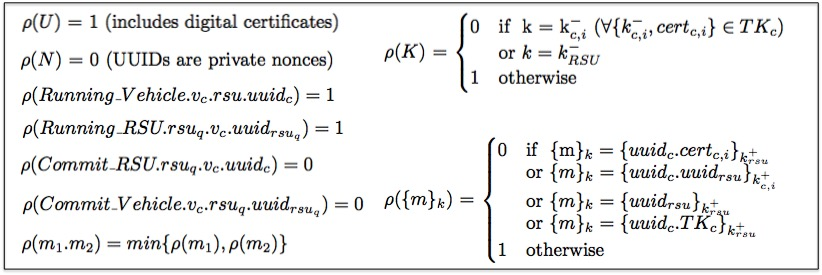
\includegraphics[width=10cm, height=4cm]{figures/rankfunctionvalues.jpg}
\caption{
A Rank function for the proposed pseudonym renewal protocol.}
\label{fig:rankfunction}
\end{figure}

The properties of the Rank Function Theorem are as follows. At each property, we describe the analysis of the pseudonym renewal protocol.

\begin{itemize}
	\item Property 1 - $\forall~m \in IK \cdot \rho(m) > 0$: this property states that the intruder knowledge may only have positive rank. In our case, the set IK contains all public digital certificates, such as the $i^{th}$ digital certificate $cert_{c, i}$ of any vehicle $v_c$ or $cert_{RSU}$, that all correspond to public keys (and also represent vehicle identities or pseudonyms). There is nothing in this set that is of non-positive rank. Therefore, the condition is satisfied; 
	
	\item Property 2 -  $\forall~S \subseteq \mathcal{M}, m \in \mathcal{M} \cdot ( (\forall~m' \in S \cdot \rho(m') > 0) \wedge S \vdash m) \Rightarrow \rho(m) > 0$: this property states that a set of positive rank messages may only  generate positive rank messages. In our case, any positive rank message allows an intruder to guess a non-positive rank message. The four messages of non-positive rank - in the subcases $\rho(\{m\}_k)$ are encrypted under public keys, which their correspondent private keys are also non-positive. This avoids the \textit{Intruder} from sending these four messages - and also from find out the nonce values, which are also non-positive. Thus, this condition is also satisfied;
	
	\item Property 3 - $\forall~t \in T \cdot \rho(t) \leq 0$: this property states that none of the events in \textit{T} can be of positive rank. In our case, both signal events $Commit\_RSU.rsu_q.v_c.uuid_{c} \in T$ and $Commit\_Vehicle.v_c.rsu_q.uuid_{rsu_q} \in T$ are of non-positive rank. Hence, this condition is satisfied;
	
	\item Property 4 - $\forall a \in \mathcal{U} \cdot PART_{a}~\underset{R}{\|}~\textit{Stop}~\textbf{sat}$ maintain positive $\rho$: this property states that every process in the \textit{SYSTEM} needs to maintain $\rho$ while being restricted on the events in set \textit{R}. In our case, $Running\_Vehicle.v_c.rsu.uuid_c \in R$ and $Running\_RSU.rsu_q.v_c.uuid_{rsu_q} \in R$. Thus, we need to verify if the two communicating process maintain $\rho$. The restriction on \textit{Vehicle} process is as follows:
	
	
	$Vehicle_{c} \underset{Running\_Vehicle.v_{c}.rsu_{q}}{\|}~\textit{Stop} = $ \parbox[t]{.6\textwidth}{$\Box_{b} \\ 
	send.v_{c}.rsu_{b}.\{uuid_c.cert_{c,i}\}_{k^{+}_{RSU}} \rightarrow \\ 
	receive.v_{c}.rsu_{b}.\{uuid, uuid_{rsu}\}_{k^{+}_{c, i}} \rightarrow \\ 
	if~rsu_b = rsu_q \wedge uuid = uuid_c~then\\
	STOP \\
	else~Running\_Vehicle.v_{c}.rsu_q.uuid_{rsu} \rightarrow \\
	send.v_{c}.rsu.\{uuid_{rsu}\}_{k^{+}_{RSU}} \rightarrow STOP$} \\
		
	In the choice operator $\Box_b$, \textit{b} represents the other participants that vehicle $v_{c}$ may communicate with. According to the modified process described above, if $uuid \neq uuid_c$, then the vehicle $v_{c}$ is not enabled to transmit $\{uuid_{rsu}\}_{k^{+}_{RSU}}$. Hence, the RSU will never run the correspondent commit signal ($Commit\_RSU.rsu_q.v_c.uuid_{rsu}$). Therefore, \textit{SYSTEM} maintains positive rank and the vehicle authenticates the current RSU.
	In order to RSU authenticate a given vehicle $v_{c}$, the same modified process is made in the \textit{RoadSide} process, such as follows.
	\\
	
	$RoadSide_{q} \underset{Running\_RSU.rsu_{q}.v_{c}}{\|}~\textit{Stop} = $ \parbox[t]{.6\textwidth}{$\Box_{b} \\ 
	receive.rsu_{q}.v_{b}.\{uuid_b, cert_{b, i}\}_{k^{+}_{RSU}} \rightarrow \\
	send.rsu_{q}.v_{b}.\{uuid_b.uuid_{rsu_q}\}_{k^{+}_{b, i}} \rightarrow \\ 
	receive.rsu_{q}.v_b.\{uuid_b, uuid\}_{k^{+}_{RSU}} \rightarrow \\ 
	if~v_b = v_c \wedge uuid = uuid_{rsu_q}~then\\
	STOP \\
	else~Running\_RSU.rsu_{q}.v_{b}.uuid_{b} \rightarrow \\
	send.rsu_q.v_b.\{uuid_b.TK_b\}_{k^{+}_{b, i}} \rightarrow STOP$} \\
	
	As previously detailed, in the choice operator $\Box_b$, \textit{b} represents the other participants that RSU $rsu_{q}$ may communicate with. if $uuid \neq uuid_{rsu_q}$, then the RSU $rsu_{q}$ is not enabled to transmit $\{TK_b\}_{k^{+}_{b, i}}$. Hence, the vehicle will never run the correspondent commit signal ($Commit\_Vehicle.v_c.rsu_q.uuid_{c}$). Therefore, \textit{SYSTEM} maintains positive rank and the RSU authenticates the current vehicle $v_{c}$.
	
	Finally, as detailed in Equation~\ref{eq:systemsatisfystop}, the  \textit{SYSTEM} is proved to satisfy such specification, and the protocol is proved to be correct for the property of authentication. As seen in the analysis above, when the signal \textit{Running} is prevented from occurring in \textit{SYSTEM}, then the following signal \textit{Commit} was not possible in \textit{SYSTEM}. Thus, \textit{Commit} does not appear in any trace \textit{tr} of \textit{SYSTEM}.
	
\end{itemize}

%Finally, according to the Equations IV, V, IX and X, they accomplish the verification correctness together. 



%s, as deeply discussed by Yang et al~\cite{yang2006limitation}

%One of the most important threat to security is called \textit{man-in-the-middle} (MITM) attack. A successful MITM attack, within our context, would result in two vehicles - $v_{c}$ and a malicious vehicle $v_{attacker}$ - to store the same set of temporary key pairs $TK_{c == attacker}$. Therefore, the attacker would explore network attacks on behalf of $v_{c}$ (but $v_{attacker}$ could also be prosecuted and identified based on the group signature $\sigma$, without compromising $v_{c}$'s reliability).
%
%We informally describe that our authentication protocol is secure against MITM in two levels, as detailed as follows: suppose a malicious vehicle $v_{attacker}$ (insider) eavesdrops on the wireless channel and intercepts $v_{c}$'s request message $m_{c}$. Therefore, it generates a new request message $m_{attacker}$ by signing $\sigma$ as $payload = UUID_{attacker} || cert_{attacker, i}$. After receiving $m_{attacker}$ and validating it, the RSU generates the new set $TK_{attacker}$ and sends it back, combined with $UUID_{attacker}$. In addition, to complete the attack, $v_{attacker}$ must return to $v_{c}$ the new set $TK_{attacker}$ as following: $E(k^{+}_{c, i}, TK_{c = attacker} || UU\\ID_{c})$. However, $v_{attacker}$ can not encrypt the whole message with the $i^{th}$ $v_{c}$'s public key ($k^{+}_{c,i}$), since $v_{attacker}$ can not capture $cert_{c, i}$ from the original message $m_{c}$. On the other hand, suppose that $v_{attacker}$ captured $cert_{c, i}$ (when $v_{c}$ attached it on earlier messages) and extracted $k^{+}_{c, i}$. Even so, the attacker would have to find out the $v_{c}$'s random value $UUID_c$, which is impossible since $v_{attacker}$ does not have RUS's private key. Moreover, the UUID identifier is 128-\textit{bit} longer, thus, the probability that an attacker would have to find out $UUID_c$ would be $1/2^{128}$ (or $q/2^{128}$, for \textit{q} guesses), which is strictly small.

%In this section, we formally verify the correctness of the pseudonym renewal protocol (Phase 2) based on the BAN logic, which is a formal logic used to reason about beliefs, encryption, and protocols. The following four postulates of the BAN logic were used in order to prove the correctness of the proposed protocol. Let P and Q be two abstract entities, while X and Y are formulas:
%
%\begin{enumerate}
%\renewcommand{\theenumi}{\Alph{enumi}}
%	\item ${\displaystyle \frac{P \vDash Q \overset{Y}{\rightleftharpoons} P, P \triangleleft <X>Y}{P \vDash Q \mid\thicksim X}}$;
%	
%	\item ${\displaystyle \frac{P \vDash \#(X), P \vDash Q \mid\thicksim X }{P \vDash Q \vDash X}}$;
%
%	\item ${\displaystyle \frac{P \vDash Q \Rightarrow X, P \vDash Q \vDash X }{P \vDash X}}$;	
%	
%	\item ${\displaystyle \frac{P \vDash \#(X)}{P \vDash \#(Y,X)}}$.
%\end{enumerate}
%
%Table~\ref{tab:idealizedprotocol} summarizes the idealized protocol in BAN Logic syntax, with the following nomenclatures: Y is the $i^{th}$ $v_{c}$'s temporary digital certificate $cert_{c,i} \in Tk_{c, w}$; Z is the $i^{th}$ $v_{c}$'s public key $k^{+}_{c,i} \in cert_{c, i}$; X denotes the request on Step 1 of the proposed pseudonym renewal protocol; and, finally, P represents the new set of temporary public/private key pairs $Tk^{'}_{c, w}$ to vehicle $v_{c}$.
%
%\begin{center}
%\tablefirsthead{%
%\hline
%\multicolumn{1}{|c}{Steps} &
%\multicolumn{1}{c|}{BAN Description} \\
%\hline}
%\tablehead{%
%\hline
%\multicolumn{2}{|l|}{\small\sl continued from previous page}\\
%\hline
%\multicolumn{1}{|c}{Steps} &
%\multicolumn{1}{c|}{BAN Description} \\
%\hline}
%\tabletail{%
%\hline
%\multicolumn{2}{|r|}{\small\sl continued on next page}\\
%\hline}
%\tablelasttail{\hline}
%\vspace{2cm}
%\topcaption{Idealized Protocol.}
%\begin{supertabular}{|l@{\hspace{3mm}}|l@{\hspace{37mm}}|}
%\label{tab:idealizedprotocol}
%  Step 1 & $v_{c} \rightarrow RSU_{n}: <X>Y$\\
%  Step 3 & $RSU_{n} \rightarrow v_{c}: \{P\}_{Z}$ \\
%\end{supertabular}
%\end{center}
%
%The Steps 1 through 8 bellow describe the assumptions considered to the verification process, while Table~\ref{tab:goals} summarizes the goals of correctness verification. The goal is to check if the vehicle and RSU trust the received messages. In other words, if the request is fresh and, hence, it is not originated from replay attacks, as well as if the message's data are authentic.
%
%\begin{enumerate}
%	\item $RSU_{n} \vDash v_{c} \overset{Y}{\rightleftharpoons} RSU_{n}$;
%	\item $RSU_{n} \vDash \#(X)$;
%	\item $RSU_{n} \vDash v_{c} \Rightarrow X$;
%	\item $RSU_{n} \triangleleft <X> Y$;
%	\item $v_{c} \triangleleft <P>Z$;
%	\item $v_{c} \vDash RSU_{n} \overset{Z}{\rightleftharpoons} v_{c}$;
%	\item $v_{c} \vDash RSU_{n} \Rightarrow P$;
%	\item $v_{c} \vDash \#(P)$.
%\end{enumerate} 
%
%\begin{center}
%\tablefirsthead{%
%\hline
%\multicolumn{1}{|c}{Goal} &
%\multicolumn{1}{|c|}{BAN Syntax} &
%\multicolumn{1}{c|}{Description} \\
%\hline}
%\tablehead{%
%\hline
%\multicolumn{2}{|l|}{\small\sl continued from previous page}\\
%\hline
%\multicolumn{1}{|c}{Goal} &
%\multicolumn{1}{|c|}{BAN Description} &
%\multicolumn{1}{c|}{Description} \\
%\hline}
%\tabletail{%
%\hline
%\multicolumn{2}{|r|}{\small\sl continued on next page}\\
%\hline}
%\tablelasttail{\hline}
%\topcaption{Goals of the Correctness Verification.}
%
%\begin{supertabular}{|l@{\hspace{3mm}}|l@{\hspace{5mm}}|l|}
%\label{tab:goals}
%  1 & $RSU_{n} \vDash X$ & RSU believes the request \textit{m}.\\ \hline
%  2 & $RSU_{n} \vDash \#(Y,X)$ & \pbox{20cm}{RSU believes that the \\ request \textit{m} and the $v_{c}$'s \\ digital certificate are fresh.}  \\ \hline
%  3 & $v_{c} \vDash P$ & \pbox{20cm}{$v_{c}$ believes the new set of \\ pseudonym.}\\ \hline
%  4 & $v_{c} \vDash \#(P,Z)$ & \pbox{20cm}{$v_{c}$ believes that the RSU \\ response is fresh.} \\
%\end{supertabular}
%\end{center}
%
%The verification process is as follows:
%
%\begin{enumerate}
%\renewcommand{\theenumi}{\Roman{enumi}}
%	\item Postulate A applied to assumptions 1 and 4:
%	 
%		${\displaystyle \frac{RSU_{n} \vDash v_{c} \overset{Y}{\rightleftharpoons} RSU_{n}, RSU_{n} \triangleleft <X>Y}{RSU_{n} \vDash v_{c} \mid\thicksim X}}$: if RSU believes that it shares the secret Y with vehicle $v_{c}$, and it receives the request X combined with Y, then it believes that $v_{c}$ once sent X;
%	
%	\item Postulate B applied to assumption 2 and to result I:
%	
%		${\displaystyle \frac{RSU_{n} \vDash \#(X), RSU_{n} \vDash v_{c} \mid\thicksim X }{RSU_{n} \vDash v_{c} \vDash X}}$: if RSU believes that the request X could have been uttered only recently (through the message timestamp), and the RSU believes that the vehicle $v_{c}$ once sent X (due to the $i^{th}$ digital certificate $cert_{k, i}$), then the RSU believes that $v_{c}$ believes X;
%	
%	\item Postulate C applied to assumption 3 and result II: 
%	
%		${\displaystyle \frac{RSU_{n} \vDash v_{c} \Rightarrow X, RSU_{n} \vDash v_{c} \vDash X }{RSU_{n} \vDash X}}$: if the RSU believes that the vehicle $v_{c}$ has jurisdiction over X (due to the $i^{th}$ digital certificate $cert_{c, i}$), and RSU trusts $v_{c}$ on the truth of X, then, RSU trusts X. Hence, goal 1 is achieved;
%		
%	\item Postulate D applied to assumption 2: 
%		
%		${\displaystyle \frac{RSU \vDash \#(X)}{RSU \vDash \#(Y,X)}}$: if the RSU believes that the request X is fresh, then the entire message is also fresh. Hence, goal 2 is achieved;
%
%\item Postulate A applied to assumptions 5 and 6:
%	
%		${\displaystyle \frac{v_{c} \vDash RSU_{n} \overset{Z}{\rightleftharpoons} v_{c}, v_{c} \triangleleft <P>Z}{v_{c} \vDash RSU \mid\thicksim P}}$: if the vehicle $v_{c}$ believes that it shares its public key Z with the RSU, and it receives the set of new public/private key pairs P from RSU combined with Z, then the vehicle $v_{c}$ believes that RSU once sent P;
%		
%	\item Postulate B applied to assumption 8 and to result V:
%		
%		${\displaystyle \frac{v_{c} \vDash \#(P), v_{c} \vDash RSU_{n} \mid\thicksim P }{v_{c} \vDash RSU_{n} \vDash P}}$: if the vehicle $v_{c}$ believes that the new set of public/private key pairs P could have been uttered only recently, and the $v_{c}$ believes that the RSU once sent P, then $v_{c}$ believes that the RSU believes P;
%	
%	\item Postulate C applied to assumption 7 and to result VI:
%	
%		${\displaystyle \frac{v_{c} \vDash RSU_{n} \Rightarrow P, v_{c} \vDash RSU_{n} \vDash P}{v_{c} \vDash P}}$: if vehicle $v_{c}$ believes that the RSU has jurisdiction over the new set of public/private key pairs P (once the RSU digitally signs each key pair), and the vehicle $v_{c}$ trusts RSU on the truth of P, then $v_{c}$ trusts P. Hence, goal 3 is achieved;
%		
%	\item Postulate D applied to assumption 8:
%	
%	${\displaystyle \frac{v_{c} \vDash \#(P)}{v_{c} \vDash \#(P,Z)}}$: if the vehicle $v_{c}$ believes the set of new public/private key pairs P is fresh (once each key pair digital certificate also carries a timestamp), then the whole formula is also fresh. That is, the RSU response message is also fresh. Hence, goal 4 is achieved.
%\end{enumerate}
%
%Finally, according to the Equations III, IV, VII and VIII, they accomplish the verification correctness together. 

\subsection{Analysis of Anonymous Communication}
\label{sec:anonymousanalisis}

The \textit{anonymity} of a vehicle means that the vehicle is not identifiable within a set of vehicles, the vehicles' anonymity set. A system with N active vehicles, the maximum degree of anonymity is achieved when an eavesdropper sees all vehicles equally probable as being the originator of a message. Therefore, we applied a normalized Shannon's Entropy method~\cite{diaz2002information} in order to quantify the uncertainty of information and to evaluate the degree of anonymity of the vehicles in a geographical area.

We compare the entropy of the anonymity set compared to the maximum entropy of the system after a vehicle exposed its $i^{th}$ level anonymity set digital certificate. Therefore, we compare how distinguishable this vehicle is within the set of possible vehicles if an eavesdropper sees its network messages in a given location.

Equation~\ref{eq:maximumentropy} defines the maximum entropy $H^{M}_{AS_{i,j}}$ of a given vehicles' anonymity set $AS_{i,j}$. Let $N_{AS_{1,j}}$ be the number of vehicles in the anonymity set $AS_{1,j}$ (first level).

\begin{equation} 
\label{eq:maximumentropy}
H^{M}_{AS_{1,j}} = log_{2}(N_{AS_{1,j}})
\end{equation}

Equation~\ref{eq:entropyafterattack} defines the anonymity set entropy $H^{X}_{AS_{i,j}}$ after a vehicle exposed its $i^{th}$ level anonymity set digital certificate. An eavesdropper assigns $p_{v_c}$ as the probability that a vehicle $v_{c}$ sent a specific message.

\begin{equation} 
\label{eq:entropyafterattack}
H^{X}_{AS_{i,j}} = - \sum_{k=1}^{N} log_{2} (p_{v_c})
\end{equation}

The information the eavesdropper has learned after observing the $i^{th}$ anonymity set digital certificate is $H^{M}_{AS_{1,j}}  - H^{X}_{AS_{i,j}}$. We divide by $H^{M}_{AS_{1,j}}$ to normalize the value. Therefore, Equation~\ref{eq:anonymityequation} defines the degree of anonymity $d_{AS_{i, j}}$ of a specific vehicles' anonymity set $AS_{i,j}$:

\begin{equation} 
\label{eq:anonymityequation}
d_{AS_{i, j}} = 1 - \frac{H^{M}_{AS_{1,j}} - H^{X}_{AS_{i,j}}}{H^{M}_{AS_{1,j}}} = \frac{H^{X}_{AS_{i,j}}}{H^{M}_{AS_{1,j}}}
\end{equation}

The degree of anonymity $d_{AS_{i, j}}$ ranges between 0 - when a vehicle appears as being the originator of messages with probability 1 - and 1 - when all vehicles that belong to the anonymity set $AS_{i, j}$ appear as being the originator with the same probability. 

Table~\ref{tab:degreeresults} presents an analysis of the proposed anonymous communication. We considered 80 million\footnote{According to the Brazilian's Natinal Traffic Department, at the end of 2014, this number includes cars, motorcycles and buses.} vehicles, 420 groups/level and each vehicle in 20 groups/level. The \textit{number of vehicles together per group} means that those vehicles in the same anonymity set of the first level ($AS_{1, j}$) are still together in level $i$. Therefore, when $i = 6$, all vehicles satisfy property 4 of the proposed multilevel architecture.

\begin{longtable}{ p{.10\textwidth} p{.40\textwidth}  p{.10\textwidth} p{.10\textwidth}} 
\caption{Simulation parameters.} % needs to go inside longtable environment
\label{tab:degreeresults} \\ \hline
Level & $N^{\circ}$ of vehicles together & $H^{X}_{AS_{i,j}}$ & $d_{AS_{i,j}}$ \\
\hline
\endfirsthead
\multicolumn{4}{c}%
{\tablename\ \thetable\ -- \textit{continued from previous page}} \\
\hline
Level & $N^{\circ}$  of vehicles together/group & $H^{X}_{AS_{i,j}}$ & $d_{AS_{i,j}}$ \\
\hline
\endhead
\hline \multicolumn{4}{r}{\textit{continued on next page}} \\
\endfoot
\hline
\endlastfoot
\textit{i} = 1 & 3.809.524 & 21.87 & 1.00 \\ 
\textit{i} = 2 & 181.405 & 17.47 & 0.79 \\ 
\textit{i} = 3 & 8.638 & 13.08 & 0.59  \\ 
\textit{i} = 4 & 412 & 8.7 & 0.39  \\ 
\textit{i} = 5 & 19 & 4.4 & 0.20 \\ 
\textit{i} = 6 & $\approx 1$ & -0.10 & 0.00
\end{longtable}


When a vehicle $v_{c}$ sends a message with its first level anonymity set digital certificate, its degree of anonymity is equal to 1, which means that if an attacker eavesdrops on the wireless channel, all vehicles in that group $AS_{1, j}$ appear as being the originator of the message with the same probability. As long as a vehicle $v_{c}$ attaches its $i^{th}$ anonymity set digital certificate on the beacon messages, the system exposes $v_{c}$'s anonymity ($d_{AS_{i,j}}$) smoothly. When $v_{c}$ sends all current anonymity set digital certificates ($CERT^{t}_{AS_{c}}$) in a given time interval \textit{t}, its anonymity degree is equal to zero, and $v_{c}$ appears as being the originator of that message with probability 1.

On the other hand, when vehicle $v_{c}$ exposes one anonymity set digital certificate per level ($CERT^{t}_{AS_{c}}$), it only exposed part of its anonymity. Vehicle $v_{c}$ may select another combination of current anonymity set digital certificates $CERT^{t'}_{AS_{c}}$ among all $20^6$ possibilities (for this scenario). This approach makes vehicle's privacy violation a difficult task. In addition, the probability that any two vehicles $v_{a}$ and $v_{b}$ in $AS_{1, j}$ will choose the same digital certificate of the $m - 1$ lower levels is ${\displaystyle \prod_{i=1}^{m-1}  \frac{1}{20}}$, which is very low. Therefore, the probability that a vehicle $v_{c}$ will expose its $m$ anonymity set digital certificates is also very low.

\subsection{Sybil Attack Detection Evaluation Results}
The \textit{sybil} detection evaluation aimed to answer three questions:

%If two different vehicles $v_{i}$ and $v_{j}$ are in the transmission range of each other ($v_{i}$, $v_{j} \in V_{l}$), and both belong to the same anonymity sets (considering property 4 of the multilevel anonymity set architecture), w

\begin{enumerate}
 \item What is the average time one $v_{k} \in V_{l}$ takes to decide that  messages are from two different vehicles, and not from a (potential) \textit{sybil} node?

 \item What is the average time one vehicle takes to detect a \textit{sybil} attack from \textit{beacon} messages?

\item What are the false-positive (a legitimate node is evaluated as \textit{sybil}) and false-negative (a \textit{sybil} node was not evaluated as one) detection rates?
\end{enumerate}

The simulation was performed by using the Veins simulation environment, Table~\ref{tab:simulation-parameters} summarizes the simulation parameters. 

\begin{longtable}{ p{.40\textwidth} p{.50\textwidth} } 
\caption{Simulation parameters.} % needs to go inside longtable environment
\label{tab:simulation-parameters} \\ \hline
Parameter & Value  \\
\hline
\endfirsthead
\multicolumn{2}{c}%
{\tablename\ \thetable\ -- \textit{continued from previous page}} \\
\hline
Parameter & Value  \\
\hline
\endhead
\hline \multicolumn{2}{r}{\textit{continued on next page}} \\
\endfoot
\hline
\endlastfoot
Total number of executions & 900 \\ 
Simulation Duration & between 10s to 120s\\
MAC and PHY protocols & 802.11p\\
Transmission Power & 20mW\\
Bit rate & 18Mbps\\
Beacon rates & 3, 5, and 10 beacon/s\\
Number of Vehicles & 3, 5, 7, 12, 17, 22, 25, 30, 40, ..., 100\\
Mobility model & Krauss \\
Average vehicle speed & between 15 m/s and 22 m/s\\
Anonymity set levels (\textit{m}) & 4, 5 and 6\\
\end{longtable}

Figures~\ref{fig:resultados-nao-sybil} and \ref{fig:resultados-sybil} illustrate the experimental results (average time on 95\% confidence intervals) for the first and the second questions, considering 100 \textit{ms}, 200 \textit{ms} and 300 \textit{ms} beacon message transmission intervals. This experimental approach is based on the assumption that it is possible to send beacons as frequently as possible but without overloading the communication channel~\cite{sommer2011traffic}. The solution adaptively updates the beacon frequency based on the importance of messages and based on the available capacity of the wireless channel.

%\begin{figure}[!hb]
%     \centering
%     \subfloat[Average detection time for two suspects and 10 packets per second (100 \textit{ms} beacon interval).]{\includegraphics[width=2.5in]{figures/grafico-resultados-nao-sybil-100-en.pdf}\label{fig:grafico-resultados-nao-sybil-100-en}} 
%     \subfloat[Average detection time for two suspects and 5 packets per second (200 \textit{ms} beacon interval).]{\includegraphics[width=2.5in]{figures/grafico-resultados-nao-sybil-200-en.pdf}\label{fig:grafico-resultados-nao-sybil-200-en}}
%     \subfloat[Average detection time for two suspects and 3 packets per second (300 \textit{ms} beacon interval).]{\includegraphics[width=2.5in]{figures/grafico-resultados-nao-sybil-300-en.pdf}\label{fig:grafico-resultados-nao-sybil-300-en}} \\
%     \caption{The average time to detect two benign vehicles in the transmission range. The vehicles belong to the same $m - 1$ anonymity sets (detection time in seconds and confidence level of 95\%).}
%\label{fig:resultados-nao-sybil}
%\end{figure}

%The experiments considered the worst scenarios for a given level \textit{m} of the proposed multilevel anonymity set architecture. Thus, the anonymity sets digital certificates from two vehicles were different only at the anonymity set of the last level. In this context, Equation~\ref{eq:sybil-detection-eq} was satisfied only at Levels 4, 5 or 6. 

\begin{figure}[H]%
\centering
\subfloat[]{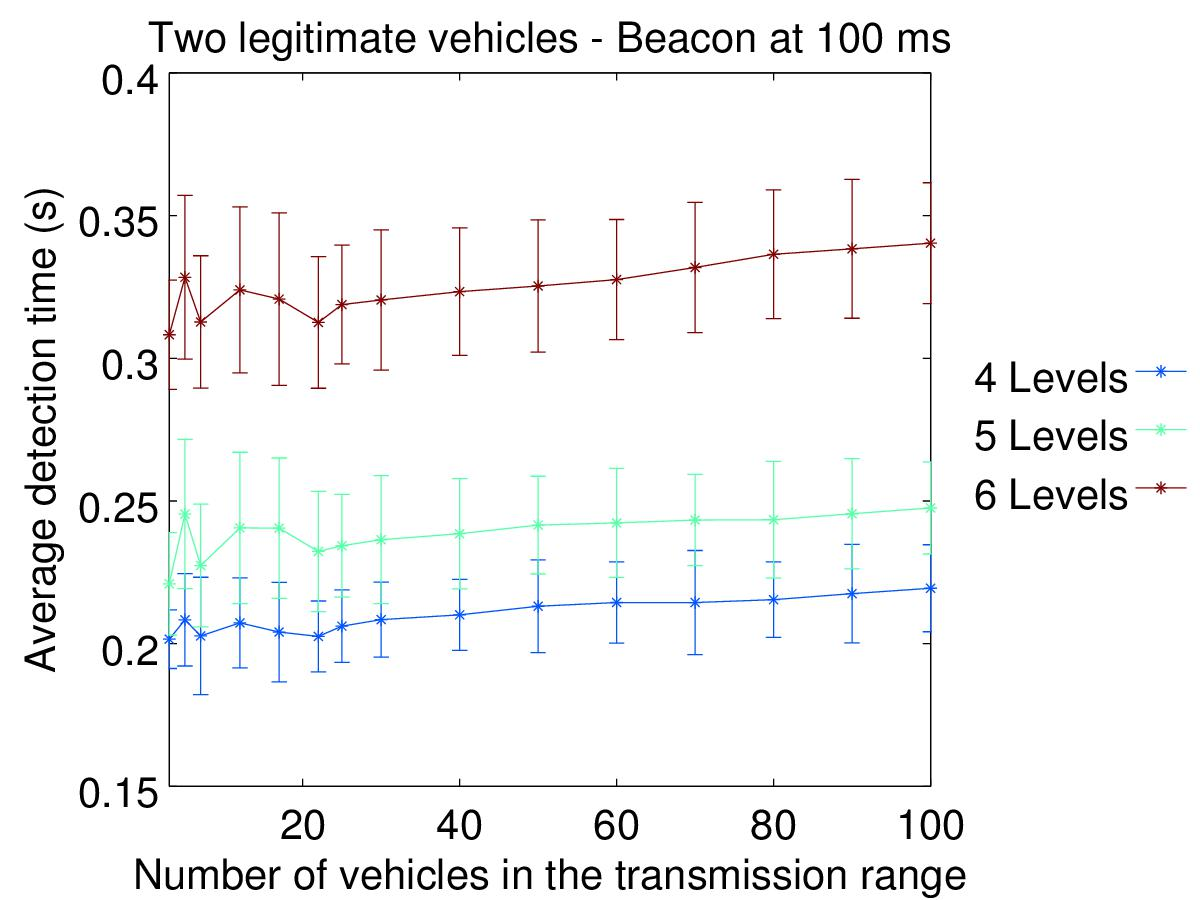
\includegraphics[scale=.28]{figures/grafico-resultados-nao-sybil-100-en-final.jpg}\label{fig:grafico-resultados-nao-sybil-100-en}}\hspace{.5cm}%
\subfloat[]{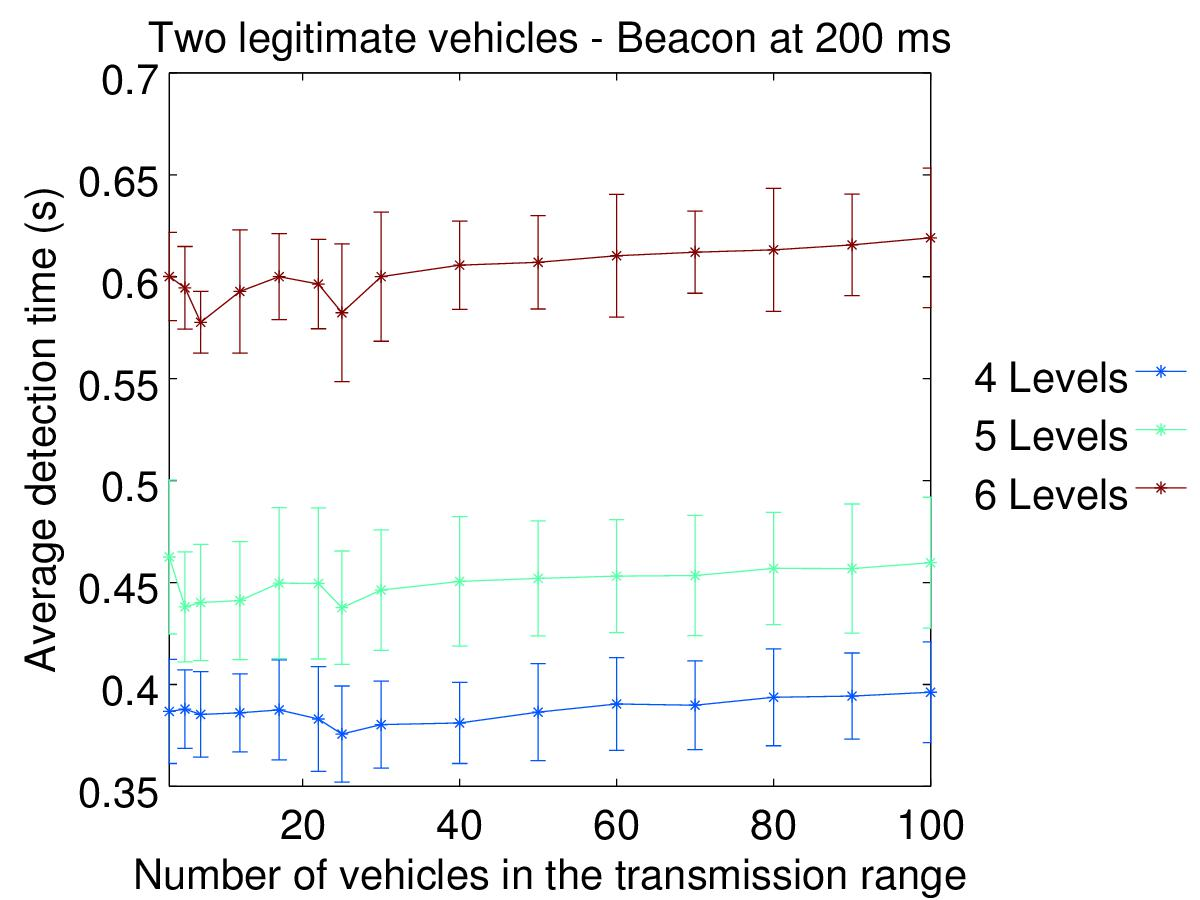
\includegraphics[scale=.28]{figures/grafico-resultados-nao-sybil-200-en-final.jpg}\label{fig:grafico-resultados-nao-sybil-200-en}}\\
\subfloat[]{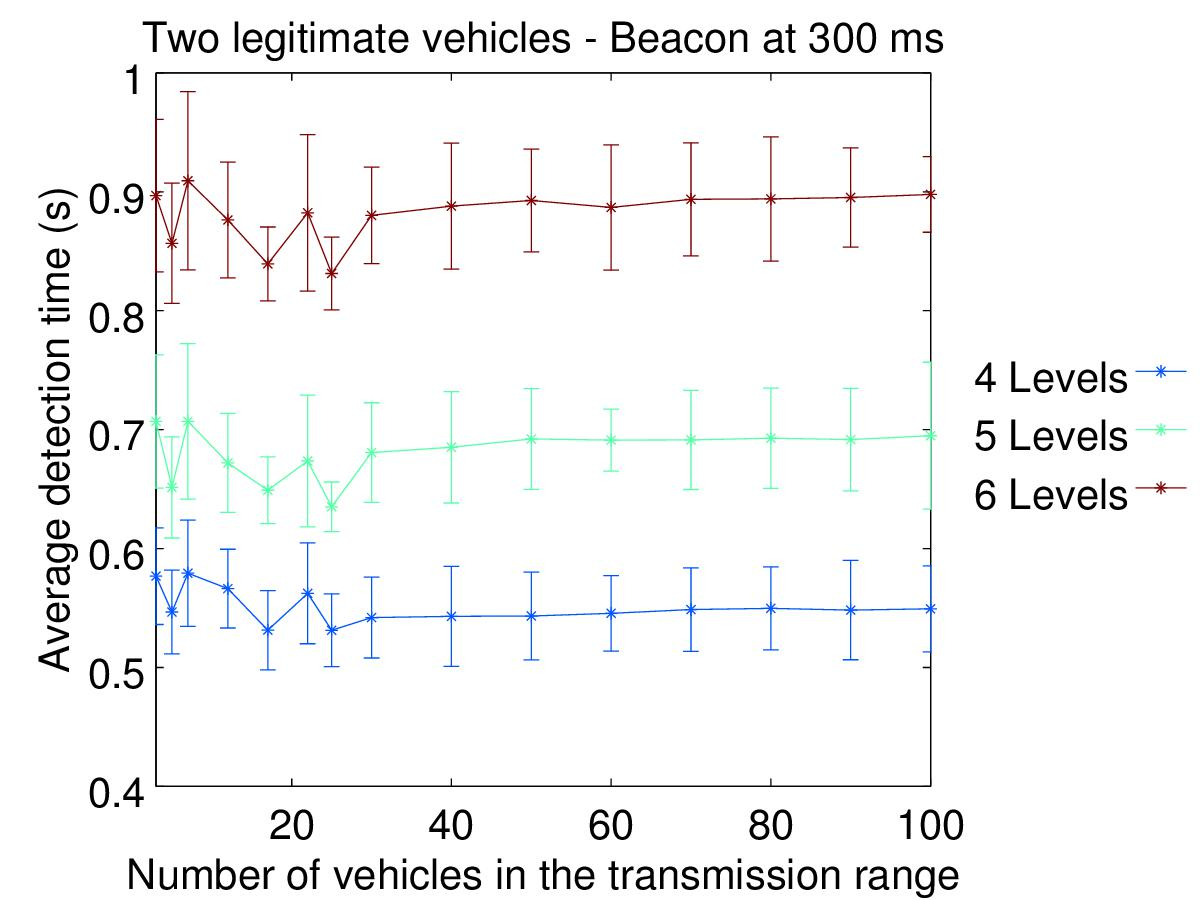
\includegraphics[scale=.28]{figures/grafico-resultados-nao-sybil-300-en-final.jpg}\label{fig:grafico-resultados-nao-sybil-300-en}}
\caption{\footnotesize{The average time to detect two legitimate vehicles in the transmission range. The vehicles belong to the same $m - 1$ anonymity sets.}}
\label{fig:resultados-nao-sybil}
\end{figure}

Figures~\ref{fig:grafico-resultados-nao-sybil-100-en}, \ref{fig:grafico-resultados-nao-sybil-200-en} and \ref{fig:grafico-resultados-nao-sybil-300-en} depict the average time to detect two legitimate vehicles that belong to the same anonymity set at Levels 3, 4, or 5 for 100, 200, and 300 beacon intervals, respectively. In short, the time to detect was lower than 0.4, 0.7, and 1 second, respectively. Since the contention is expected to be higher as the number of vehicles increases, the impact on the results was quite minimal. Moreover, the \protocolname~has low impact on the V2V communication standard mainly due to two reasons: first, the vehicles at the same anonymity sets update to the last anonymity set level fast; and the probability that two or more vehicles, in the same transmission range, will choose the same $m-1$ anonymity set digital certificates ($CERT^{t}_{AS_{v}}$) is ${\displaystyle \prod_{i=1}^{m-1}  \frac{1}{k}}$, which is very low (e.g. $k = 20$). Therefore, the proposed approach provides a stable average of detection time as the number of nodes increases. 

\begin{figure}[H]%
\centering
\subfloat[]{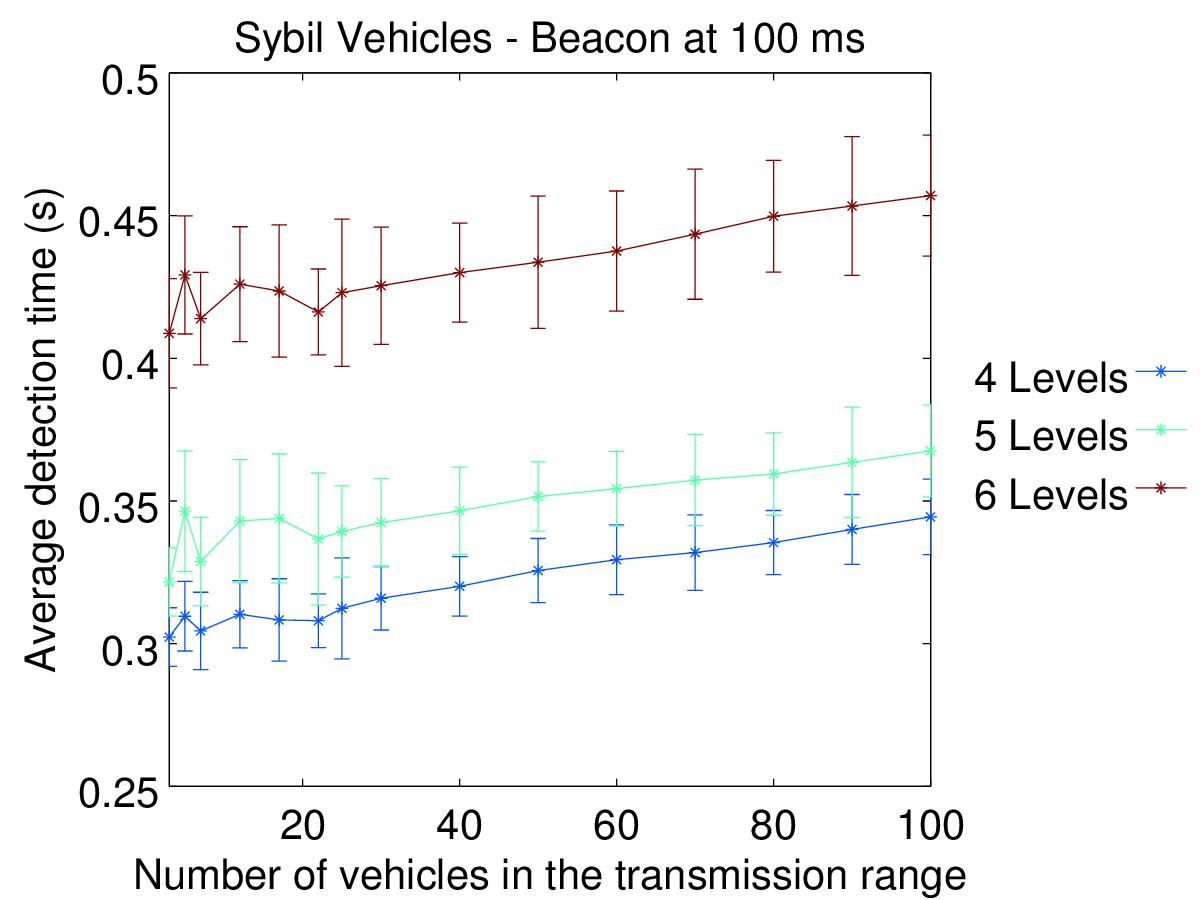
\includegraphics[scale=.28]{figures/grafico-resultados-sybil-100-en-final.jpg}\label{fig:grafico-resultados-sybil-100-en}}\hspace{.5cm}%
\subfloat[]{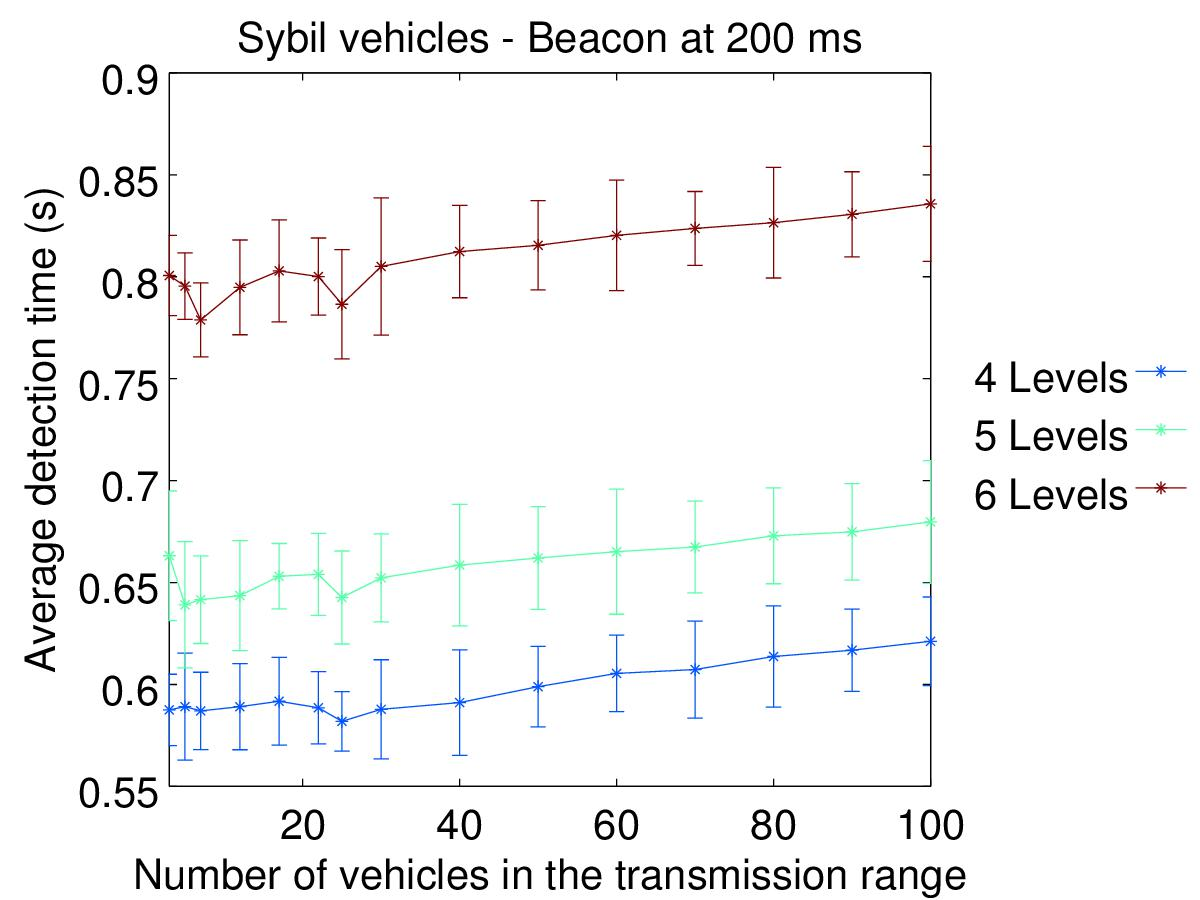
\includegraphics[scale=.28]{figures/grafico-resultados-sybil-200-en-final.jpg}\label{fig:grafico-resultados-sybil-200-en}}\\
\subfloat[]{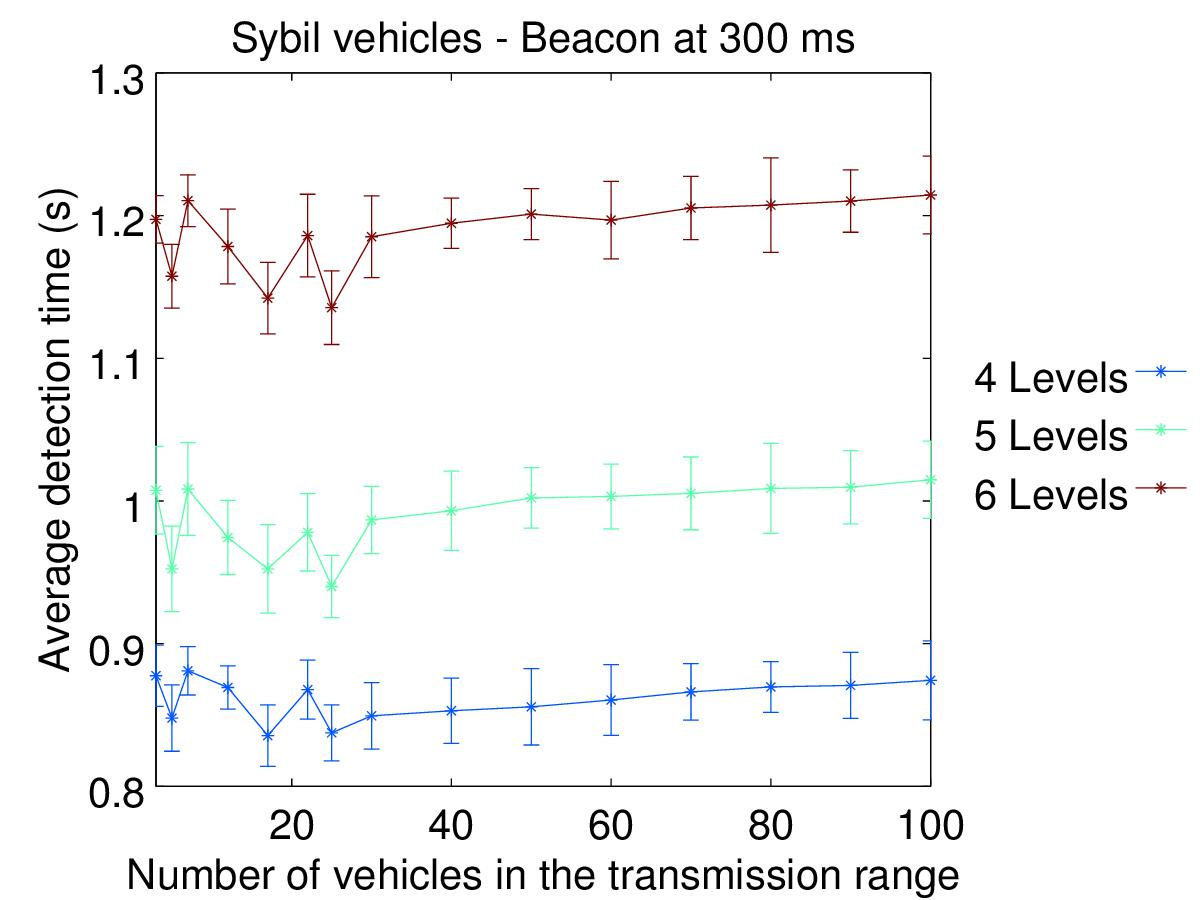
\includegraphics[scale=.28]{figures/grafico-resultados-sybil-300-en-final.jpg}\label{fig:grafico-resultados-sybil-300-en}}
\caption{\footnotesize{The average time to detect a \textit{sybil} vehicle when another legitimate vehicle in the transmission range belongs to the same $m - 1$ anonymity sets.}}
\label{fig:resultados-sybil}
\end{figure}

Figures~\ref{fig:grafico-resultados-sybil-100-en}, \ref{fig:grafico-resultados-sybil-200-en} and \ref{fig:grafico-resultados-sybil-300-en} depict the average time to detect a \textit{sybil} vehicle with three different identities. Similarly, the wireless contention had minimum impact as the number of vehicle increases. On the other hand, the results exceeded 1 second for 300 \textit{ms} beacon interval at Levels 5 and 6. This happens since the neighbor vehicles must evaluate Equation~\ref{eq:wait-time} in order to wait for the next anonymity set digital certificates before deducing a \textit{sybil} attack.

Finally, the main parameters that may affect the \textit{sybil} detection are the beacon time intervals and the number of anonymity sets (per level) in which two or more vehicles together belong to. The results are considered acceptable since the messages from a \textit{sybil} vehicle are dropped (and kept for future purposes) by neighboring vehicles during the attack, and the average detection time is faster than other approaches (as discussed on next section). The proposed approach is totally resilient to \textit{false-negative} and \textit{false-positive} results because any given vehicle may not send messages that describe the same event with different anonymity set digital certificates.

%Moreover, most of the safety-based applications for VANETs require fast drivers' reactions (e.g., \textit{blind spot} scenarios) and therefore, they demand fast decision protocols.

 %(property 4 of the proposed anonymity set multilevel architecture). Moreover, a set of messages that describe the same event and contain the same set of anonymity set digital certificate are kept as suspected by the neighboring vehicles. For instance, suppose that a malicious vehicle keeps sending beacon messages with different identities, but they contain only one anonymity set digital certificate. These messages are kept as suspected until Equation~\ref{eq:wait-time} is satisfied, or when Equation~\ref{eq:sybil-detection-eq} is satisfied, which leads to the prosecution phase. 


%\begin{figure}[h]
%     \centering
%     \subfloat[Average detection time for one \textit{Sybil} attacker and 10 packets per second (100 \textit{ms} beacon interval).]{\includegraphics[width=2.5in]{figures/grafico-resultados-sybil-100-en.pdf}\label{fig:grafico-resultados-sybil-100-en}}
%     \subfloat[Average detection time for one \textit{Sybil} attacker and 5 packets per second (200 \textit{ms} beacon interval).]{\includegraphics[width=2.5in]{figures/grafico-resultados-sybil-200-en.pdf}\label{fig:grafico-resultados-sybil-200-en}}
%     \subfloat[Average detection time for one \textit{Sybil} attacker and 3 packets per second (300 \textit{ms} beacon interval).]{\includegraphics[width=2.5in]{figures/grafico-resultados-sybil-300-en.pdf}\label{fig:grafico-resultados-sybil-300-en}}
%     \caption{The average time to detect a \textit{sybil} vehicle when another benign vehicle in the transmission range belongs to the same $m - 1$ anonymity sets (detection time in seconds and confidence level of 95\%).}
%\label{fig:resultados-sybil}
%\end{figure}

%The other two evaluated metrics were the \textit{false-positve} and \textit{false-negative} \textit{sybil} detection rates. Figure~\ref{fig:false-positive-result-scenario} depicts a scenario in which  the former metric was evaluated in 0,28\% of the experimental cases. It is a classical hidden terminal scenario where vehicles \textit{C} and \textit{A} belong to the same first level anonymity set (e.g.: $AS_{1,2}$). The vehicle \textit{B} receives beacon messages from the vehicles \textit{C} and \textit{A}. However, due to the \textit{A}'s and \textit{C}'s transmission ranges, neither \textit{A} nor \textit{C} receive the messages from each other. Therefore, they keep sending messages with their first level anonymity set digital certificate $cert_{AS_{1,2}}$. From the \textit{B}'s perspective, since the vehicles \textit{A} and \textit{C} keep sending messages without presenting the next anonymity set digital certificates, after $\delta$ \textit{ms} (Equation~\ref{eq:wait-time}), \textit{B} evaluates \textit{A}'s and \textit{C}'s messages as originated from a \textit{sybil} vehicle. However, both A and C are two benign vehicles.
%
%\begin{figure}[ht]
%\centering
%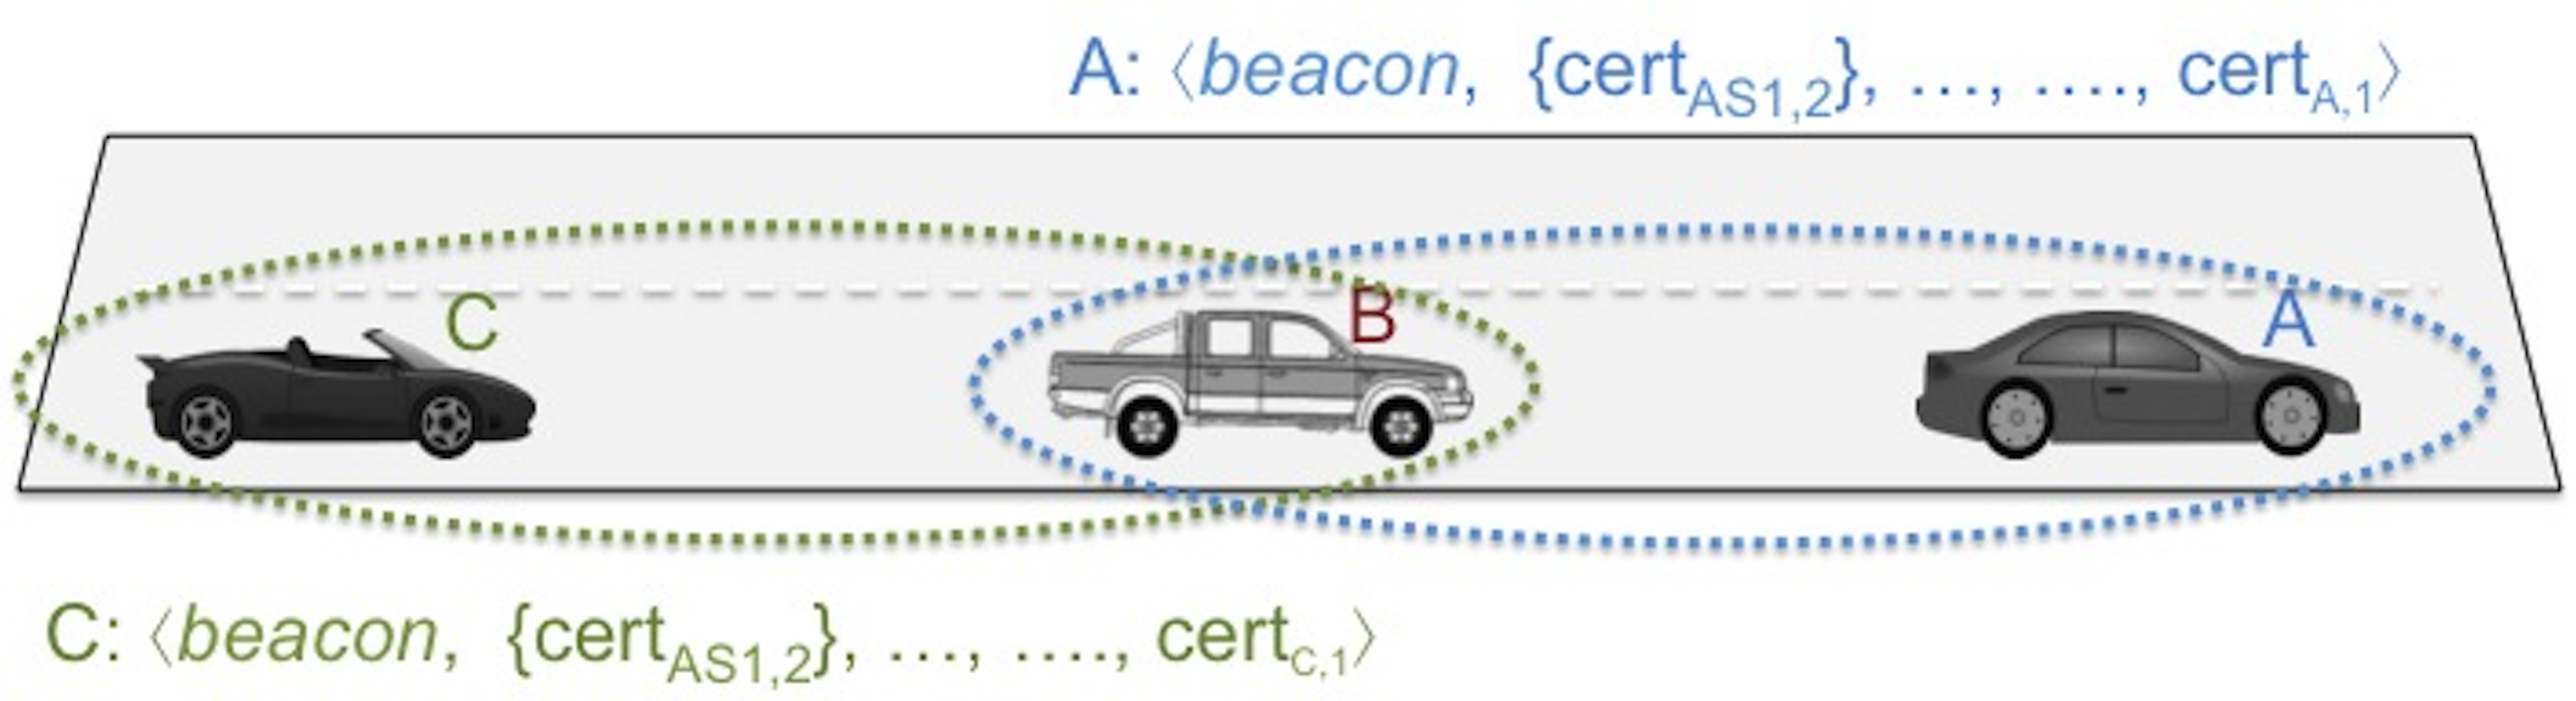
\includegraphics[scale=.45]{figures/false-positive-scenario.jpg}
%\caption{Hidden terminals scenarios may lead to false-positive \textit{sybil} detections.}
%\label{fig:false-positive-result-scenario}
%\end{figure}

\section{Related Work}
\label{sec:related}

To the best of our knowledge, Lin et al~\cite{lin2007gsis} proposed one of the most efficient group-based authentication for VANETs. In such approach, each vehicle signs the whole message with its group signing key, and may verify the sender's message authenticity by using the group public key. However, the verification process based on group signatures are slower than traditional asymmetric key pairs, which reduces the message verification rate. For instance, it takes 8.5 \textit{ms} on average to verify any received message. Therefore, a vehicle may only verify 125 messages/s, which is very low in high traffic jam. In addition, the verification process does not consider the revocation lists, which is also time-consuming and is proportional to the number of revoked vehicles.  The \protocolname~protocol uses traditional public/private key pairs for message verification, which increases the verification rate. 

Still within the context of group signature, Wu et al.~\cite{wu2010balanced} propose an efficient \textit{sybil}-proof threshold authentication for VANETs. A message is viewed as trustworthy only after it has been endorsed by at least \textit{t} vehicles, where \textit{t} is a threshold. Since the approach requires a subset of other vehicles for message verification, it may suffer from message loss and delay. On the other hand, \protocolname~will have any message delay or loss if the number of vehicles in the communication range is above 250, which will not be feasible due to communication channel overhead. Therefore, vehicles will decrease its signal strength in order to reduce channel errors due to signal collisions and overheads.   

%, malicious users may launch and explore \textit{sybil} attacks in different types of networks, such as \textit{peer-to-peer} (P2P)~\cite{sybil}, sensor~\cite{sybil-survey3}, and mobile ad hoc networks~\cite{sybil-neighborhood1}. Moreover, the attack may compromise many types of applications, such as voting~\cite{tran2012combating}, reputation systems~\cite{reputation-sybil2}, as well as distributed storage and resource sharing systems~\cite{xiao2007security}, to name a few. Thus, there have been many approaches to avoid and detect \textit{sybil} attacks. 
%
%Initially, Douceur~\cite{sybil} proposed the resource testing method. In short, Douceur's assumption requires that each physical entity is limited in resources such as computation, storage and communication. Hence, a \textit{sybil} entity would not perform a set of tasks in a given time interval as expected if these identities would belong to different entities. However, in ad hoc networks, one node may have more computational resources than other nodes. Similarly, in sensor networks, the radio resource testing, proposed by Newsome~\cite{sybil-survey3}, assumes that each physical entity has only one radio resource and is able to send and receive only on one channel simultaneously. This cannot be a realistic assumption on VANET.

With respect to the \textit{sybil} attack detections, Zhou et al.~\cite{p2dap2, p2dap} propose a privacy-preserving \textit{sybil} attack detection protocol called $P^{2}DAP$. To detect a \textit{sybil} attack, the approach needs the RSU and the CA. The drawback of such approach is that a \textit{sybil} attacker will not be detected if there are no RSUs around. Hence, the approach is highly dependent on the RSU deployment methods and its availability (e.g.: DoS attack may compromise V2V communications). Moreover, experimental results show that a \textit{sybil} detection may achieve 20 seconds due to high overhead imposed on RSUs, which is a high average time for real world on-road services. 

%First, a CA provides to every vehicle a pool of pseudonyms that are used for preserving the vehicle's privacy. To prevent \textit{sybil} attacks, the pseudonyms assigned to a particular vehicle are hashed to a common value called \textit{coarse-grained hash value}. Afterwards, the same pseudonyms are hashed to another hash value called \textit{fine-grained hash value}. Vehicles with the same coarse-grained values are grouped together, while the pseudonyms with fine-grained values are unique to each vehicle. 

%On the other hand, our approach does not need a fixed infrastructure to avoid or detect \textit{sybil} attacks and, as well as for the same number of vehicles and \textit{sybil} attacker (e.g.: 90 vehicles, and one \textit{sybil} vehicle), our approach detects the \textit{sybil} attack faster than $P^{2}DAP$.

%an RSU captures the messages sent from the vehicles along a road and verifies the \textit{course-grained hash values}. If two or more messages have the same \textit{coarse-grained hash values}, the RSU forwards the messages to the CA. The CA then verifies the \textit{fine-grained hash values} and checks if these values are also the same. If it evaluates to true, this vehicle is malicious (a \textit{sybil} vehicle).

Another strategy for detecting \textit{sybil} attacks is based on a timestamp series approach~\cite{sybil-time-space1, sybil-time-stamp1}. The approach explores the relationship between time and space, where two or more vehicles will not pass nearby the same RSU and send requests to it at the same time. This approach may compromise users' privacy since it requires vehicle authentication at each RSU, which allows third-party entities to assemble a vehicle routing profile. In addition, the scheme cannot be applied directly to an urban environment with a very complex roadway infrastructure, many signals and intersections, as deeply discussed in~\cite{sybil-time-stamp1}. Our approach does not depend on the roadway infrastructure.

%Thus, an RSU issues digitally signed timestamps to each vehicle. Then, each vehicle must attach to beacon messages at least the last two timestamps. If two different messages with different identities contain the same last two timestamps, then they belong to a \textit{sybil} vehicle. 

Finally, a \textit{sybil} detection approach may use data from neighboring vehicles to filter malicious vehicles~\cite{sybil-neighborhood1, sybil-neighborhood3}. In Grover's et al. approach~\cite{sybil-neighborhood2}, every vehicle builds a neighboring table (which contains vehicles' identities) with different time interval. After this process, each vehicle shares its neighboring table with other vehicles. If every vehicle has the same neighbors' identities for different time intervals, then these identities may belong to the same (\textit{sybil}) vehicle. Nonetheless, a \textit{sybil} vehicle may never be detected (\textit{false-negative} results) if it changes its identities between consecutive time intervals. As previously discussed, our approach does not provide \textit{false-negative} detections. To sum up, if different vehicles stay together for a long period of time, then it results in \textit{false-positive} \textit{sybil} detections.

We compare our proposed privacy-preserving \textit{sybil} detection protocol to other similar approaches on Table~\ref{tab:comparison}. The main advantage of our scheme is its resilience to both \textit{false-negative} and \textit{false-positive} detections without a centralized infrastructure during detection time, which imposes less overhead on RSUs. In addition, it decreases the average time to detect \textit{sybil} attacks. The dependency on a centralized infrastructure may also compromise VANET services if a more sophisticated network attack also makes such infrastructure unavailable. 

\begin{longtable}{ p{.05\textwidth} p{.17\textwidth} p{.14\textwidth} p{.08\textwidth} p{.18\textwidth} p{.14\textwidth} } 
\caption{Comparison to other approaches.}
 % needs to go inside longtable environment
\label{tab:comparison} \\ \hline
 & \pbox{20cm}{False-Positive \\ False-Negative \\ Resilient} & \pbox{20cm}{Non-\\Repudiation}  & \pbox{20cm}{Beacon \\ or \\ Event} & \pbox{20cm}{Infrastructure-\\Dependent}  & \pbox{20cm}{Roadway \\ Infrastructure- \\Dependent } \\
\hline
\endfirsthead
\multicolumn{6}{c}%
{\tablename\ \thetable\ -- \textit{continued from previous page}} \\
\hline
 & \pbox{20cm}{False-Positive \\ False-Negative \\ Resilient} & \pbox{20cm}{Non-\\Repudiation}  & \pbox{20cm}{Beacon \\ or \\ Event} & \pbox{20cm}{Infrastructure-\\Dependent}  & \pbox{20cm}{Roadway \\ Infrastructure- \\Dependent } \\
\hline
\endhead
\hline \multicolumn{6}{r}{\textit{continued on next page}} \\
\endfoot
\hline
\endlastfoot

Our & \textbf{Both} & Yes & Both & \textbf{No} & No\\ 
\cite{p2dap2} & Negative & Yes & Both & Yes & No\\
\cite{sybil-time-space1} & None & * & Both & Yes & Yes \\ 
\cite{sybil-time-space2} & None & * & Both & Yes & Yes \\ 
\cite{sybil-time-stamp1} & None & No & Both & Yes & Yes \\ 
\cite{sybil-neighborhood2} & None & * & Beacon & No & No \\ 
\cite{sybil-neighborhood3} & None & * & Beacon & No & No \\

\end{longtable}

\section{Conclusion and Future Work}
\label{sec:conclusion}

In this paper we have presented a privacy-preserving authentication and \textit{sybil} detection protocol for vehicular ad hoc networks called~\protocolname. In order to provide users' privacy, the protocol provides a multilevel anonymity set architecture, with group signature and pseudonyms. The experimental results show its secure and efficiency. Moreover, \protocolname~is also resilient to \textit{false-negative} and \textit{false-positive} detections without the support of centralized infrastructures during \textit{sybil} attack detection time. As future work, in order to avoid the RSU from forwarding each single prosecution message to the CA, the RSU must first evaluate if the messages belong to the same \textit{sybil} detection process. This will avoid a CA from measuring redundant prosecution messages. Both V2I communications are still being evaluated.

The challenge in detecting \textit{sybil} attacks in VANETs resides in the potential threats to users' privacy, since during \textit{sybil} detection time, multiple identities must be linked to a one single, yet non-malicious, entity. On the other hand, when a CA may not be always available in VANETs, a potential solution for detecting \textit{sybil} attacks must consider only the vehicles in the region of attack, where  each vehicle must share control data in order to detect the attack. 
%According to Douceur~\cite{sybil}, without a logically, yet trusted centralized authority (CA), which will vouch for a one-to-one correspondence between entity and identity, \textit{sybil} attacks are always possible except under extreme and unrealistic assumptions of resource parity and coordination among entities.

%The V2I communication type is the most important communication type that still must be evaluated. Vehicles and RSUs communicate to negotiate new sets of pseudonyms, as well as during the prosecution phase. The communication overhead, w.r.t. the network traffic, of both depends on the number of vehicles that send the renewal or prosecution messages to a given RSU. The former is a kind of \textit{three-way-handshake} protocol, which, at a first glance, does not impose high overhead on RSUs due to the low probability that a high number of vehicles need to change the set of pseudonyms at the same time. The last one tends to impose a high overhead on RSUs if there is a high number of vehicles that made part of a \textit{sybil} detection process at the same region and they send prosecution messages to the same RSU. 
%As another future work, we are evaluating the achieved degree of anonymity of a given anonymity set $AS_{i,j}$. In other words, we would like to measure the probability of a malicious entity, which controls several sensors that are scattered across an entire city, to build a vehicle's route profile of a specific distance (e.g.: 3 \textit{km}) while the vehicle exposes the anonymity sets that it belongs to. Therefore, we are measuring a number of anonymity sets \textit{k} (for each level) that a vehicle must belong to in order to minimize the probability of the user's privacy violations. Based on the concepts of Shannon's entropy~\cite{shannon} and rough set theory~\cite{Dai201372}, as well as on the model to quantify the degree of anonymity of a set of users grouped in several subsets~\cite{diaz2002information}, the anonymity of a given anonymity set $AS_{i,j}$ may be evaluated. Therefore, it is also possible to define how vehicles may be allocated into the anonymity sets in order to maximize users' privacy with a low impact on message processing and data management overheads.

The security aspects are one of the biggest forthcoming challenges for actually deploying the concepts of VANET. The reliability of the whole system may not be compromised due to the high impact it has on people's lives. In this context, among other security-related concepts, authentication, non-repudiation, user's privacy control, and \textit{sybil} attack detections play key roles in vehicular environments and, therefore, they have gained a special attention from the research community.


%
%\begin{figure}
%
%\begin{minipage}{.5\linewidth}
%\centering
%\subfloat[]{\label{main:a}\includegraphics[scale=.35]{figures/grafico-resultados-nao-sybil-100-en.pdf}}
%\end{minipage}%
%\begin{minipage}{.5\linewidth}
%\centering
%\subfloat[]{\label{main:b}\includegraphics[scale=.35]{figures/grafico-resultados-nao-sybil-100-en.pdf}}
%\end{minipage}\par\medskip
%\centering
%\subfloat[]{\label{main:c}\includegraphics[scale=.35]{figures/grafico-resultados-nao-sybil-100-en.pdf}}
%
%\caption{my fig}
%\label{fig:main}
%\end{figure}


%% \linenumbers

%% main text


%% The Appendices part is started with the command \appendix;
%% appendix sections are then done as normal sections
%% \appendix

%% \section{}
%% \label{}

%% If you have bibdatabase file and want bibtex to generate the
%% bibitems, please use
%%
\bibliographystyle{elsarticle-num} 
\bibliography{biblio}

%% else use the following coding to input the bibitems directly in the
%% TeX file.

%\begin{thebibliography}{00}
%
%% \bibitem{label}
%% Text of bibliographic item
%
%\bibitem{}
%
%\end{thebibliography}
\end{document}
\endinput
%%
%% End of file `elsarticle-template-num.tex'.
